\documentclass[dvipsnames, svgnames, x11names]{beamer}
\usetheme{mytheme2024}
% \special{dvipdfmx:config z 0} %取消PDF压缩，加快速度，最终版本生成的时候最好把这句话注释掉
 
\title{化学反应工程}
\subtitle{第三章\ 釜式反应器}
\author{张斌}
\institute[理工系]{河北农业大学 理工系}
\date{\the\year 年 \the\month 月}
%-----------------------------------------------------------------
\begin{document}

\maketitle

	\begin{frame}{}
        \begin{center}
            {\Huge \cbf{目 \ 录}}
        \end{center}
		\tableofcontents
		\thispagestyle{empty}
		\addtocounter{framenumber}{-1}
	\end{frame}


    \section{釜式反应器的物料衡算式}


    \begin{frame}{釜式反应器}
        \qquad 釜式反应器是工业上应用最广泛的反应器之一。在本章中，只研究均相反应或者可按均相反应对待的多相反应问题。
        \begin{itemize}
          \item 既可以用来进行均相反应(主要是液相均相反应)，又可用于多相反应，如气液、液固、液液及气液固等反应。
          \item 在操作方式上，可以是连续反应，也可以间歇或半间歇操作。
          \item 釜内设有搅拌装置，因此可以认为反应区内反应物料的浓度均一，温度均一。
          \item 如果反应区内存在两个或两个以上的相态，则各相的反应物料组成未必相同，温度也不一定相等，这时各相间就可能存在质量传递和热量传递，这是进行多相反应时所必须考虑的问题。
        \end{itemize}
        
    \end{frame}
    
    
    \begin{frame}{釜式反应器的物料衡算式}
        \qquad 设在釜式反应器中进行$M$个均相反应，描述该反应系统所需要的关键组分数为$K$，$K\le M$。如果这$M$个反应均是独立的，则$K=M$。
        \\\qquad 前已假定反应器内反应物料浓度及温度处处相同，且与流出物料的相应值相等，故可取整个反应体积$V_\mathrm{r}$作控制体积。这种情况下只有时间自变量，设在时间间隔$\mathrm{d}t$内，反应器里关键组分$i$量的变化为$\mathrm{d}n_i$，如图所示，反应器进出口的物料体积流量分别为$Q_0$和$Q$，因之在时间间隔$\mathrm{d}t$内，进出反应器的关键组分量分别为$Q_0c_{i0}\mathrm{d}t$及$Qc_{i}\mathrm{d}t$，关键组分的反应量则为$\mathcal{R}_iV_\mathrm{r}\mathrm{d}t$。
        \begin{columns}[c]
            \column{9.75cm}
                根据质量守恒定律有
                $$Q_0c_{i0}\mathrm{d}t=Qc_{i}\mathrm{d}t-\mathcal{R}_iV_\mathrm{r}\mathrm{d}t+\mathrm{d}n_i$$
                若$i$为反应物，$\mathcal{R}_i$为负；反应产物的$\mathcal{R}_i$则为正。
            \column{3.75cm}
                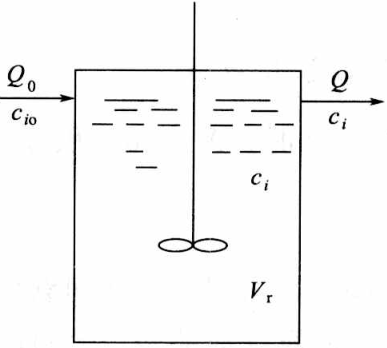
\includegraphics[height=2.5cm]{figs/fig3.1.png}
        \end{columns}
    \end{frame}
    
    
    \begin{frame}{釜式反应器的物料衡算式}    
        $$Q_0c_{i0}=Qc_{i}-\mathcal{R}_iV_\mathrm{r}+\mathrm{d}n_i/\mathrm{d}t \qquad (i=1,2,\cdots,K)$$
        \\这就是釜式反应器的物料衡算式，是一组常微分方程。关键组分$i$在反应器内的累积速率$\mathrm{d}n_i/\mathrm{d}t$可正可负，视具体情况而定。
        \\定态下操作的反应器，累积速率为零，
        $$Q_0c_{i0}=Qc_{i}-\mathcal{R}_iV_\mathrm{r} \qquad (i=1,2,\cdots,K)$$
        此为连续釜式反应器的物料衡算式，为一个代数方程组。
        \\如果采用间歇操作，无物料的输入与输出，即$Q_0=Q=0$，
        $$-\mathcal{R}_iV_\mathrm{r}+\mathrm{d}n_i/\mathrm{d}t=0 \qquad (i=1,2,\cdots,K)$$
        此为间歇釜式反应器的物料衡算式，为一组常微分方程。
    \end{frame}


    \section{等温间歇釜式反应器的计算(单一反应)}


\begin{frame}
    \frametitle{间歇反应器的特点}
    \begin{minipage}{0.68\linewidth}
        间歇反应器最根本的特点是所有操作步骤（投料、反应、出料）都是分批、间歇式进行的。
    \begin{itemize}
      \item \bf{一次性投料：}在反应开始前，将所有反应物一次性加入反应器中。
      \item \bf{间歇式反应：}在反应过程中，没有物料流入或流出。反应器成为一个封闭系统，反应物在设定的条件（如温度、压力、搅拌速度）下进行反应，直到达到预期的转化率或反应时间。
      \item \bf{一次性出料：}反应结束后，将整个反应混合物（包括产物和未反应的物料）一次性排出，然后进行清洗，为下一批生产做准备。
      \end{itemize}
    \end{minipage}\hfill
    \begin{minipage}{0.28\linewidth}
        \begin{figure}[htpb]
            \centering
            
\includegraphics[width=.9\linewidth]{高压锅}
            \caption{高压锅炖肉}
        \end{figure}
    \end{minipage}
\end{frame}


\begin{frame}
    \frametitle{间歇反应器的优缺点}
    \begin{minipage}{0.48\linewidth}
        主要优点：
        \begin{itemize}
          \item \bf{操作灵活性强}，同一台设备可以很方便地用于生产不同的产品，只需改变投料配方、反应温度、压力和反应时间即可。
          \item \bf{适用于慢反应}：对于反应速率很慢的反应，可以给予足够的反应时间。
          \item \bf{高转化率}：由于反应物在反应器内有充分的停留时间，可以很容易地达到很高的转化率。
        \end{itemize}
    \end{minipage}\hfill
    \begin{minipage}{0.48\linewidth}
        主要缺点：
        \begin{itemize}
          \item \bf{生产效率低}：由于投料、升温、降温、出料、清洗等辅助操作需要占用大量时间，导致设备的有效利用率不高。
          \item \bf{劳动强度大或自动化成本高}：传统的间歇操作需要大量的人工干预。
          \item \bf{规模放大有挑战}：大反应釜的传热面积与体积之比变小，可能导致升温/降温困难。
        \end{itemize}
    \end{minipage}
\end{frame}


\begin{frame}
    \frametitle{间歇反应器的典型应用}
    间歇反应器非常适合小批量、多品种的生产，如精细化工、医药、染料等行业。
    \begin{itemize}
      \item \bf{精细化工行业：}生产品种繁多、批量小的产品，如颜料、染料、添加剂、特种化学品等。
      \item \bf{制药工业：}尤其是原料药（API）的生产，通常涉及复杂的多步合成，且批量相对较小，对灵活性要求极高。
      \item \bf{食品工业：}如酿造啤酒、生产酱料等。
      \item \bf{高分子工业：}某些特殊牌号的聚合物生产，如乳液聚合。
      \item \bf{研究与开发：}在实验室中，几乎所有的化学反应探索和工艺优化最初都是在间歇反应器（如圆底烧瓶、高压反应釜）中进行的。
    \end{itemize}
\end{frame}


\begin{frame}{等温间歇釜式反应器的计算}
    设计间歇反应器的关键就在于确定每批所需时间。由于间歇反应器是分批操作，其操作时间系由两部分组成：
    \begin{enumerate}
      \item \bf{反应时间}，即装料完毕后算起至达到所要求的产品收率时所需时间；
      \item \bf{辅助时间}，即装料、卸料及清洗等所需时间之和。
    \end{enumerate}
    其中尤以反应时间的确定最为重要，而辅助时间主要根据经验来确定。
    \[
        \mathrm{\bf{总操作时间 = 反应时间 + 辅助时间}}
    \]
\end{frame}


\begin{frame}{反应时间的计算}      
    设反应器中进行化学反应\ce{A + B -> R}，并以A为关键组分。若反应开始时关键组分的量为$n_\mathrm{A0}$，则
    $$n_{\mathrm{A}}=n_{\mathrm{A} 0}(1-X_{\mathrm{A}})$$
    $$-V_{\mathrm{r}} \mathscr{R}_{\mathrm{A}}-n_{\mathrm{A} 0} \frac{\mathrm{d} X_{\mathrm{A}}}{\mathrm{d} t}=0$$        
    当$t=0$时，$X_\mathrm{A}=0$，积分上式即可求A的转化率到$X_\mathrm{Af}$时所需的反应时间
    $$t=\int_{0}^{X_{\mathrm{Af}}} \frac{n_{\mathrm{A} 0} \mathrm{~d} X_{\mathrm{A}}}{V_{\mathrm{r}}(-\mathscr{R}_{\mathrm{A}})}$$
    上式适用于任何间歇反应过程：多相还是均相，等温或非等温。
\end{frame}


\begin{frame}{反应时间的计算}      
    对于等容过程，反应混合物体积$V_\mathrm{r}$可视为常数。若为均相反应，$n_{\mathrm{A0}}/V_\mathrm{r}=c_{\mathrm{A0}}$，
    $$t=c_{\mathrm{A} 0} \int_{0}^{X_{\mathrm{Af}}} \frac{\mathrm{d} X_{\mathrm{A}}}{(-\mathscr{R}_{\mathrm{A}})}$$
    对于单一反应，$(-\mathscr{R}_\mathrm{A}=r_\mathrm{A})$，所以只要反应的速率方程已知，代入上式便可计算关键组分A的转化率达到$X_\mathrm{Af}$时所需的时间。对于单一反应，间歇反应器反应时间的求定是直接积分反应速率方程的结果。反应时间的长短取决于反应组分的初始浓度（一级反应除外）和所要求达到的最终转化率。当然，这是指反应温度一定而言，反应温度不同，反应时间当然也不一样。
\end{frame}


\begin{frame}{反应时间的计算}      
    \begin{table}        
        \caption{简单级数反应特征}
        \begin{tabular}{c l l l l}
            \Xhline{1pt}
            级数 & \makecell[c]{速率方程} & \makecell[c]{速率方程积分式}  & \makecell[c]{$t$和$c_\mathrm{A}$关系} & \makecell[c]{$t$和$X_\mathrm{A}$关系}\\
            \hline
            \rule{0pt}{16pt} 1 & $r=kc_\mathrm{A}$ & $\ln c_\mathrm{A}=-kt+\ln c_\mathrm{A0}$ & $t=\frac{1}{k}\ln\frac{c_\mathrm{A0}}{c_\mathrm{A}}$ & $t=\frac{1}{k}\ln \frac{1}{1-X_\mathrm{A}}$\\
            \rule{0pt}{16pt} 2 & $r=kc_\mathrm{A}^2$ & $\frac{1}{c_\mathrm{A}}=kt + \frac{1}{c_\mathrm{A0}}$ & $t=\frac{1}{k}(\frac{1}{c_\mathrm{A}}-\frac{1}{c_\mathrm{A0}})$ & $t=\frac{1}{kc_\mathrm{A0}} \frac{X_\mathrm{A}}{1-X_\mathrm{A}}$\\
            \rule{0pt}{16pt} 0 & $r=k$ & $c_\mathrm{A}=-kt+c_\mathrm{A0}$ & $t=\frac{1}{k}(c_\mathrm{A0}-c_\mathrm{A})$ & $t=\frac{1}{k}c_\mathrm{A0}X_\mathrm{A}$\\
            \Xhline{1pt}
        \end{tabular}
\end{table}
\begin{itemize}
  \item 一级反应的反应时间$t$与初始浓度$c_\mathrm{A0}$无关
  \item 二级反应的反应时间$t$与初始浓度$c_\mathrm{A0}$成反比
  \item 零级反应的反应时间$t$与初始浓度$c_\mathrm{A0}$成正比
\end{itemize}
\end{frame}


\begin{frame}[t]
    \frametitle{}
    \begin{example}
        蔗糖在稀水溶液中水解生成葡葡糖和果糖。当水极大过量时，反应遵循一级反应动力学。反应温度为48℃时 ， 反应速率常数$k=0.0193$ \si{min^{-1}}。当蔗糖的浓度为\SI{1}{mol/L}和\SI{5}{mol/L}时，若蔗糖的浓度降到\SI{0.01}{mol/L}时，所需反应时间各为多少？
    \tcblower
    \pause
    \[
        \begin{aligned}
            t_1&=\frac{1}{0.0193}\ln\frac{1}{0.01}=238\min \\
            t_2&=\frac{1}{0.0193}\ln\frac{5}{0.01}=322\min 
        \end{aligned}
    \]
    \end{example}
\end{frame}


\begin{frame}[t]
    \frametitle{}
    \begin{example}
        设某反应的动力学方程为$r_\mathrm{A}=0.0193c_\mathrm{A}^2$ \si{mol.L^{-1}.s^{-1}}， 当 A 的浓度分别为\SI{1}{mol/L}和\SI{5}{mol/L}时，若A 的残余浓度要求为\SI{0.01}{mol/L}，各需多长反应时间 ？
    \tcblower
    \pause
    \[
        \begin{aligned}
            t_{1}&=\frac{1}{0.0193}\times\left(\frac{1}{0.01}-\frac{1}{1}\right)=5130\mathrm{min}\\
            t_{2}&=\frac{1}{0.0193}\times\left(\frac{1}{0.01}-\frac{1}{5}\right)=5171\mathrm{min}
        \end{aligned}
    \]
    \pause
    计算表明，对于二级反应 ， 若要求残余浓度很低时 ， 尽管初始浓度相差甚大 ， 其所需反应时间相差甚小，表明反应的大部分时间花费在反应末期 。
    \end{example}
\end{frame}


% \begin{frame}{反应时间的计算}      
%     \qquad 由间歇反应器的设计方程可得一个极为重要的结论：反应物达到一定的转化率所需的反应时间，只取决于过程的反应速率，也就是说取决于动力学因素，而与反应器的大小无关。反应器的大小是由反应物料的处理量决定的。由此可见，上述计算反应时间公式，既适用于小型设备，又可用于大型设备。所以，由实验室数据设计生产规模的间歇反应器时，只要保证两者的反应条件相同，便可达到同样的反应效果。但应注意，要使两个规模不同的间歇反应器具有完全相同的反应条件并非易事，以等温间歇反应器为例，实验室用的小反应器要做到等温操作比较容易，而大型反应器就很难做到；又如实验室反应器通过搅拌可使反应物料混合均匀，浓度均一，而大型反应器要做到这一点就比较困难。因此，生产规模的间歇反应器其反应效果与实验室反应器相比，或多或少地总是会有些差异。
% \end{frame}


\begin{frame}[t]
    \frametitle{}
    \begin{question}
        在间歇操作的釜式反应器中进行己二酸（A）和己二醇（B）以等摩尔比缩聚反应生产醇酸树脂。实验测得动力学方程式为$r_\mathrm{A} = kc_\mathrm{A}^2$\ \si{kmol/(L.h)}。其中，速率常数$k = 118.2$ \ \si{L/(kmol.h)}，反应物的初始浓度$c_\mathrm{A0} = 0.005$\ \si{kmol/L}。若每天处理2400 kg己二酸，求转化率为$X_\mathrm{Af}$时所需反应时间。
        \begin{table}
            \centering
            \begin{tabular}{cc||cc}
                \bottomrule
                $X_\mathrm{Af}=0.1$ & 410\quad 411 \quad 412 & $X_\mathrm{Af}=0.7$ & 级数 \quad 奈何桥也是桥 \\ 
                $X_\mathrm{Af}=0.2$ & 421 \quad 424 \quad 425
                & $X_\mathrm{Af}=0.8$ & 压力 \quad G.T.I.大家庭  \\ 
                $X_\mathrm{Af}=0.3$ & 1 \quad 123 \quad 12138 & $X_\mathrm{Af}=0.9$ & [默认组名] \quad 没有这个组  \\ 
                $X_\mathrm{Af}=0.4$ & 227 \quad 233 \quad 241 & $X_\mathrm{Af}=0.99$ & 反应级数 \quad 哈基米典礼 \\
                $X_\mathrm{Af}=0.5$ & 413 \quad 12345 & $X_\mathrm{Af}=0.999$ & 欧内的手组 \quad 化工科技组  \\
                $X_\mathrm{Af}=0.6$ & 沉淀 \quad 新建分组 & $X_\mathrm{Af}=0.9999$ & 私人小组 \quad 没组的来  \\  \toprule
            \end{tabular}
        \end{table}
    \end{question}
\end{frame}


\begin{frame}[t]
    \frametitle{}
    \begin{question}
        在间歇操作的釜式反应器中进行己二酸（A）和己二醇（B）以等摩尔比缩聚反应生产醇酸树脂。实验测得动力学方程式为$r_\mathrm{A} = kc_\mathrm{A}^2$\ \si{kmol/(L.h)}。其中，速率常数$k = 118.2$ \ \si{L/(kmol.h)}，反应物的初始浓度$c_\mathrm{A0} = 0.005$\ \si{kmol/L}。若每天处理2400 kg己二酸，求转化率为$X_\mathrm{Af}$时所需反应时间。
        % \tcblower
        \begin{table}
            \centering
            \begin{tabular}{cc||cc||cc}
                \bottomrule
                $X_\mathrm{Af}$ & 反应时间\ (h) & $X_\mathrm{Af}$ & 反应时间\ (h) & $X_\mathrm{Af}$ & 反应时间\ (h) \\ \hline
                0.1 & 0.19 & 0.5 & 1.69 & 0.9 & 15.23 \\ 
                0.2 & 0.42 & 0.6 & 2.54 & 0.99 & 167.5 \\ 
                0.3 & 0.73 & 0.7 & 3.95 & 0.999 & 1690 \\ 
                0.4 & 1.13 & 0.8 & 6.77 & 0.9999 & 16919 \\ \toprule
            \end{tabular}
        \end{table}
    \end{question}
\end{frame}


\begin{frame}{反应体积$V_\mathrm{r}$的计算}      
    间歇反应器的反应体积$V_\mathrm{r}$取决于单位时间的反应物料处理量$Q_0$及每批生产所需的操作时间。操作时间由两部分组成：反应时间$t$和辅助时间$t_0$。
    \begin{enumerate}
      \item $Q_0$由生产任务计算得到；
      \item $t$由化学动力学所确定；
      \item $t_0$根据实际经验来决定。
    \end{enumerate}
    反应体积$V_\mathrm{r}$用下式计算：
    \[
        V_\mathrm{r}=Q_0(t+t_0)
    \]
\end{frame}


\begin{frame}
    \frametitle{反应器的体积$V$}
    反应器的体积$V$要比反应体积$V_\mathrm{r}$大，以保证反应物料上面有一定空间，一般用下式计算：
    \[
        V=\frac{V_\mathrm{r}}{f}
    \]
    \begin{table}
        \centering
        \caption{设备装料系数$f$}
        \begin{tabular}{cc}
            \bottomrule
            条件 & \qquad 装料系数$f$范围\qquad  \\ \hline
            不带搅拌或搅拌缓慢的反应釜 & $0.8\sim 0.85$ \\ 
            带搅拌的反应釜 & $0.7\sim 0.8$ \\ 
            易起泡沫和在沸腾下操作的设备 & $0.4\sim 0.6$ \\ \toprule
        \end{tabular}
    \end{table}
\end{frame}


\begin{frame}[t]
    \frametitle{}
    \begin{question}
        在间歇操作的釜式反应器中进行己二酸（A）和己二醇（B）缩聚反应。动力学方程式为$r_\mathrm{A} = kc_\mathrm{A}^2$\ \si{kmol/(L.h)}。其中，速率常数$k = 118.2$ \ \si{L/(kmol.h)}，反应物的初始浓度$c_\mathrm{A0} = 0.005$\ \si{kmol/L}。若每天处理2400 kg己二酸，每批辅助时间为1 h，反应器装填系数为0.8，求转化率为$X_\mathrm{Af}$时所需反应器的体积。
        \begin{table}
            \centering
            \begin{tabular}{cc||cc}
                \bottomrule
                $X_\mathrm{Af}=0.1$ & 410\quad 411 \quad 412 & $X_\mathrm{Af}=0.7$ & 级数 \quad 奈何桥也是桥 \\ 
                $X_\mathrm{Af}=0.2$ & 421 \quad 424 \quad 425
                & $X_\mathrm{Af}=0.8$ & 压力 \quad G.T.I.大家庭  \\ 
                $X_\mathrm{Af}=0.3$ & 1 \quad 123 \quad 12138 & $X_\mathrm{Af}=0.9$ & [默认组名] \quad 没有这个组  \\ 
                $X_\mathrm{Af}=0.4$ & 227 \quad 233 \quad 241 & $X_\mathrm{Af}=0.99$ & 反应级数 \quad 哈基米典礼 \\
                $X_\mathrm{Af}=0.5$ & 413 \quad 12345 & $X_\mathrm{Af}=0.999$ & 欧内的手组 \quad 化工科技组  \\
                $X_\mathrm{Af}=0.6$ & 沉淀 \quad 新建分组 & $X_\mathrm{Af}=0.9999$ & 私人小组 \quad 没组的来  \\  \toprule
            \end{tabular}
        \end{table}
    \end{question}
\end{frame}


\begin{frame}[t]
    \frametitle{}
    \begin{question}
        在间歇操作的釜式反应器中进行己二酸（A）和己二醇（B）缩聚反应。动力学方程式为$r_\mathrm{A} = kc_\mathrm{A}^2$\ \si{kmol/(L.h)}。其中，速率常数$k = 118.2$ \ \si{L/(kmol.h)}，反应物的初始浓度$c_\mathrm{A0} = 0.005$\ \si{kmol/L}。若每天处理2400 kg己二酸，每批辅助时间为1 h，反应器装填系数为0.8，求转化率为$X_\mathrm{Af}$时所需反应器的体积。
        % \tcblower
        \begin{table}
            \centering
            \begin{tabular}{cc||cc||cc}
                \bottomrule
                $X_\mathrm{Af}$ & 反应器体积\ (\si{m^3}) & $X_\mathrm{Af}$ & 反应器体积\ (\si{m^3}) & $X_\mathrm{Af}$ & 反应器体积\ (\si{m^3}) \\ \hline
                0.1 & 0.20 & 0.5 & 0.46 & 0.9 & 2.78 \\ 
                0.2 & 0.24 & 0.6 & 0.61 & 0.99 & 28.85 \\ 
                0.3 & 0.30 & 0.7 & 0.85 & 0.999 & 289.6 \\ 
                0.4 & 0.36 & 0.8 & 1.33 & 0.9999 & 28972 \\ \toprule
            \end{tabular}
        \end{table}
    \end{question}
\end{frame}


\begin{frame}[t]{}
    \begin{example}
        用间歇反应器进行乙酸和乙醇的酯化反应，每天生产乙酸乙酯12000kg，
            $$\ce{CH3COOH + C2H5OH <=> CH3COOC2H5 + H2O}$$
            $$(A)\qquad\qquad(B)\qquad\qquad\qquad(R)\qquad\qquad(S)$$
        原料中反应组分的质量比为A:B:S=1:2:1.35，反应液的密度为1020kg/m$^3$，并假定在反应过程中不变。每批装料、卸料及清洗等辅助操作时间为1h。反应在100℃下等温操作，其反应速率方程如下
        \vspace{-7pt}
        $$r_{\mathrm{A}}=k_{1}(c_{\mathrm{A}} c_{\mathrm{B}}-c_{\mathrm{R}} c_{\mathrm{S}} / K)$$
        100℃时，$k_1=\SI{4.76e{-4}}{L/(mol.min)}$，平衡常数$K$=2.92。试计算乙酸转化35％时所需的反应体积。根据反应物料的特性，若反应器填充系数取0.75，则反应器的实际体积是多少？
    \end{example}
\end{frame}


\begin{frame}{最优反应时间}
    间歇反应器，反应物浓度随反应时间增长而降低，反应产物的生成速率则随着反应物浓度的降低而降低。所以，随着时间的延长，产品产量增多，但按单位操作时间计算的产品产量不一定增加。
    
    对于反应\ce{A -> R}，若反应产物R的浓度为$c_\mathrm{R}$，则单位操作时间的产品产量为
    $$F_{\mathrm{R}}=\frac{V_{\mathrm{r}} c_{\mathrm{R}}}{t+t_{0}}$$
    对反应时间$t$求导
    $$\frac{\mathrm{d} F_{\mathrm{R}}}{\mathrm{d} t}=\frac{V_{\mathrm{r}}\left[(t+t_{0}) \frac{\mathrm{d} c_{\mathrm{R}}}{\mathrm{d} t}-c_{\mathrm{R}}\right]}{\left(t+t_{0}\right)^{2}}$$
    $$\text{令}\frac{\mathrm{d} F_{\mathrm{R}}}{\mathrm{d} t}=0 \qquad\text{得}\qquad \frac{\mathrm{d} c_{\mathrm{R}}}{\mathrm{d} t}=\frac{c_{\mathrm{R}}}{t+t_{0}}\qquad\text{或}\qquad \frac{\mathrm{d} X_{\mathrm{A}}}{\mathrm{d} t}=\frac{X_{\mathrm{A}}}{t+t_{0}}$$
    即为单位时间产物产量最大必须满足的条件，由此可求出最优反应时间。
\end{frame}


\begin{frame}[t]{}
    \begin{example}
        在反应体积为12.38m$^3$的间歇釜式反应器进行乙酸乙酯生产，反应动力学和反应条件同上。试求单位操作时间乙酸乙酯最大产量是多少？此时乙酸的转化率是多少？
    \end{example}
\end{frame}

\begin{frame}{最优反应时间}
    \begin{itemize}
        \item 以单位时间产品产量最大为目标函数 $$\frac{\mathrm{d} c_{\mathrm{R}}}{\mathrm{d} t}=\frac{c_{\mathrm{R}}}{t+t_{0}}$$
        \item 以单位产品所消耗原料最少为目标函数\\\qquad 反应时间越长，原料单耗越少
        \item 以生产费用最低为目标函数\\\qquad 总费用=反应操作费用+辅助操作费用+固定费用$A=a+a_0+a_\mathrm{f}$\\\qquad 单位质量产品的总费用为$$A_{\mathrm{T}}=\frac{a t+a_{0} t_{0}+a_{\mathrm{f}}}{V_{\mathrm{r}} c_{\mathrm{R}}}$$\qquad 为使$A_{\mathrm{T}}$最小，令$\frac{\mathrm{d} A_{\mathrm{T}}}{\mathrm{d} t}=0$，解之得最优反应时间。
    \end{itemize}
\end{frame}


\section{等温间歇釜式反应器的计算(复合反应)}


\begin{frame}
    \frametitle{回顾：间歇釜式反应器的物料衡算式}
    \begin{framed}
        \[
            -\mathcal{R}_iV_\mathrm{r}+\mathrm{d}n_i/\mathrm{d}t=0
        \]
    \end{framed}
\end{frame}


\begin{frame}{平行反应}
    设在等温间歇釜式反应器中进行下列平行反应，P为目的产物
    \vspace{-2pt}
    $$\begin{array}{l}
        \mathrm{A} \longrightarrow \mathrm{P}, \quad r_{\mathrm{P}}=k_{1} c_{\mathrm{A}} \\
        \mathrm{A} \longrightarrow \mathrm{Q}, \quad r_{\mathrm{Q}}=k_{2} c_{\mathrm{A}}
    \end{array}$$
    各反应组分的物料衡算式如下: 
    $$\begin{cases}
        V_{\mathrm{r}}(k_{1}+k_{2}) c_{\mathrm{A}}+\frac{\mathrm{d} n_{\mathrm{A}}}{\mathrm{d} t}=0\\
        -V_{\mathrm{r}} k_{1} c_{\mathrm{A}}+\frac{\mathrm{d} n_{\mathrm{P}}}{\mathrm{d} t}=0\\
        -V_{\mathrm{r}} k_{2} c_{\mathrm{A}}+\frac{\mathrm{d} n_{\mathrm{Q}}}{\mathrm{d} t}=0
    \end{cases}
    \quad \text{对于恒容均相系统}
    \begin{cases}
        (k_{1}+k_{2}) c_{\mathrm{A}}+\frac{\mathrm{d} c_{\mathrm{A}}}{\mathrm{d} t}=0\\
        -k_{1} c_{\mathrm{A}}+\frac{\mathrm{d} c_{\mathrm{P}}}{\mathrm{d} t}=0\\
        -k_{2} c_{\mathrm{A}}+\frac{\mathrm{d} c_{\mathrm{Q}}}{\mathrm{d} t}=0
    \end{cases}
    \begin{matrix}
        (1)\\
        (2)\\
        (3)
    \end{matrix}$$
    设$t=0$时，$c_\mathrm{A}=c_\mathrm{A0}$，$c_\mathrm{P}=0$，$c_\mathrm{Q}=0$，积分式(1)有
    $$c_{\mathrm{A}}=c_{\mathrm{A} 0} \exp [-(k_{1}+k_{2}) t] \quad \text{或}\quad t=\frac{1}{k_{1}+k_{2}} \ln \frac{c_{\mathrm{A} 0}}{c_{\mathrm{A}}} =\frac{1}{k_{1}+k_{2}} \ln \frac{1}{1-X_{\mathrm{A}}}$$
\end{frame}


\begin{frame}{平行反应}
    积分式(2)可得反应时间$t$时目的产物P的浓度
    $$c_{\mathrm{P}}=\frac{k_{1} c_{\mathrm{A} 0}}{k_{1}+k_{2}}\left\{1-\exp \left[-(k_{1}+k_{2}) t\right]\right\}$$
    由$c_{\mathrm{Q}}=c_{\mathrm{A} 0}-c_{\mathrm{A}}-c_{\mathrm{P}}$得
    $$c_{\mathrm{Q}}=\frac{k_{2} c_{\mathrm{A} 0}}{k_{1}+k_{2}}\left\{1-\exp \left[-(k_{1}+k_{2}) t\right]\right\}$$
    $$\frac{c_{\mathrm{P}}}{c_{\mathrm{Q}}}=\frac{k_{1}}{k_{2}}$$
    两种反应产物的浓度之比，在任何反应时间下均等于两个反应的速率常数之比。但要注意这个关系只有当各反应的速率方程形式相同时才成立。
\end{frame}


\begin{frame}{平行反应}
    \begin{columns}[c]
        \column{9cm}
        根据$c_{\mathrm{A}},c_{\mathrm{P}},c_{\mathrm{Q}}$浓度式可绘出示意图如图所示。
        
        由图可见，反应物A的浓度总是随反应时间的增加而减少，而反应产物P和Q的浓度则随反应时间的增加而增高。
        \column{4.5cm}
            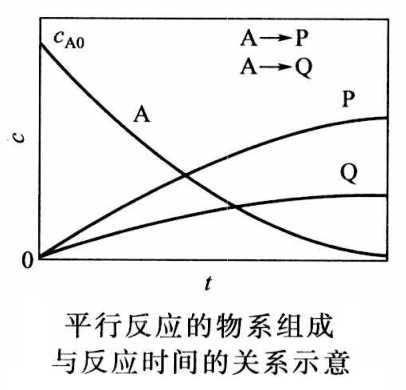
\includegraphics[width=4.5cm]{figs/fig3.2.png}
    \end{columns}
    以上是两个一级反应的情况，不难推广到M个一级反应同时进行情况
    $$c_{\mathrm{A}}=c_{\mathrm{A} 0} \exp (-t \sum_{1}^{M} k_{i}) \qquad c_{i}=\frac{k_{\mathrm{i}} c_{\mathrm{A} 0}}{\sum_{1}^{M} k_{i}}[1-\exp (-t \sum_{1}^{M} k_{i})]$$
    反应时间确定后，即可确定必需的反应体积。
\end{frame}


\begin{frame}[t]{}
    \begin{block}{例3.3}
        在等温间歇釜式反应器中进行下列液相反应
        $$\mathrm{A}+\mathrm{B} \longrightarrow \mathrm{P}, \quad r_{\mathrm{P}}=2 c_{\mathrm{A}}~~ \mathrm{kmol} /(\mathrm{m}^{3} \cdot \mathrm{h})$$
        $$ 2 \mathrm{~A} \longrightarrow \mathrm{Q}, \quad r_{\mathrm{Q}}=0.5 c_{\mathrm{A}}^{2} ~~\mathrm{kmol} /(\mathrm{m}^{3} \cdot \mathrm{h})$$
        反应开始时A和B的浓度均等于2kmol/m$^3$，目的产物为P，试计算反应时间为3h时A的转化率和P的收率。
        \tcblower
        \pause
        \begin{minipage}{0.48\linewidth}
            \[
            \begin{cases}
            -\frac{\mathrm{d} c_{\mathrm{A}}}{\mathrm{d} t}=2c_{\mathrm{A}} + c_{\mathrm{A}}^2\\
            \frac{\mathrm{d} c_{\mathrm{P}}}{\mathrm{d} t}=2c_{\mathrm{A}}
            \end{cases}
            \]
        \end{minipage}\hfill
        \begin{minipage}{0.48\linewidth}
            \[
            \begin{cases}
            t = \frac{1}{2}\ln \frac{c_{\mathrm{A0}}(2+c_{\mathrm{A}})}{c_{\mathrm{A}}(2+c_{\mathrm{A0}})}\\
            c_{\mathrm{A}} = \frac{2c_{\mathrm{A0}}}{(2+c_{\mathrm{A0}})\mathrm{e}^{2t}-c_{\mathrm{A0}}}\\
            c_{\mathrm{P}} = 2\ln \frac{2+c_{\mathrm{A0}}-c_{\mathrm{A0}}\mathrm{e}^{-2t}}{2}
            \end{cases}
            \]
        \end{minipage}
        
    \end{block}
\end{frame}


\begin{frame}[t]{}
    \begin{block}{例3.3改\quad \scriptsize{《化学反应工程》李倩，化学工业出版社，94页例3-5}}
        在等温间歇釜式反应器中进行下列液相反应
        \[
            \mathrm{~A} \longrightarrow \mathrm{P}, \quad r_{\mathrm{P}}= c_{\mathrm{A}}^{2} ~~\mathrm{mol} /(\mathrm{L} \cdot \mathrm{min})
        \]
        \[
            \quad \mathrm{A} \longrightarrow \mathrm{Q}, \quad r_{\mathrm{Q}}=2 c_{\mathrm{A}}~~ \mathrm{mol} /(\mathrm{L} \cdot \mathrm{min})
        \]
        $c_{\mathrm{A0}} = \ $ \SI{4.0}{mol.L^{-1}}， $c_{\mathrm{P0}} = c_{\mathrm{Q0}} = 0$，物料体积流量为5.0 L/min，求转化率为80\%，辅助时间6 min时，$V_\mathrm{r}$是多少？目的产物P的出口处瞬时选择性为多少？
        \tcblower
        \begin{minipage}{0.38\linewidth}
            \[
            \begin{cases}
            t = \frac{1}{2}\ln \frac{c_{\mathrm{A0}}(2+c_{\mathrm{A}})}{c_{\mathrm{A}}(2+c_{\mathrm{A0}})}\\
            c_{\mathrm{A}} = \frac{2c_{\mathrm{A0}}}{(2+c_{\mathrm{A0}})\mathrm{e}^{2t}-c_{\mathrm{A0}}}
            \end{cases}
            \]
        \end{minipage}\hfill
        \begin{minipage}{0.58\linewidth}
            \pause
            \[
            \begin{cases}
            t = \frac{1}{2}\ln \frac{4\times (2+0.8)}{0.8\times (2+4)} = 0.4 \ \mathrm{min}\\
            V_\mathrm{r} = Q_0(t + t_0) = 5\times (0.4 + 6) = 32 \ \mathrm{L}\\
            S_{\mathrm{P}} = \frac{c_{\mathrm{A}}^2}{c_{\mathrm{A}}^2+2c_{\mathrm{A}}} = \frac{0.8^2}{0.8^2+2\times 0.8} = 28.6\%
            \end{cases}
            \]
        \end{minipage}
    \end{block}
\end{frame}


\begin{frame}[t]
    \frametitle{}
    \begin{redblock}{习题3.9（分组任务）}
        在间歇反应器中等温进行下列液相均相反应 ：
        \[
            \ch{A + B -> R} \qquad r_\mathrm{R} = 1.6 c_\mathrm{A} \qquad \si{kmol.m^{-3}.h^{-1}}
        \]
        \[
            \quad \ch{2 A -> D}  \qquad r_\mathrm{D} = 8.2 c_\mathrm{A}^2 \qquad \si{kmol.m^{-3}.h^{-1}}
        \]
        式中$r_\mathrm{R}$、$r_\mathrm{D}$分别表示产物 R 及 D 的生成速率。反应用的原料为 A 与 B 的混合液， 其中 A 的浓度为 \SI{2}{kmol.m^{-3}}。
        
        （1）试计算 A 的转化率达 95\%时所需要的反应时间 。

        （2）A的转化率为95\%时，R的收率是多少？

        （3）若每天处理1000\ kmol A，反应器装填系数0.8，辅助时间0.5小时，所需反应器体积是多少？
    \end{redblock}
\end{frame}


\begin{frame}
    \frametitle{连串反应}
    \[
        \mathrm{A} \stackrel{k_{1}}{\longrightarrow} \mathrm{P} \stackrel{k_{2}}{\longrightarrow} \mathrm{Q}
    \]
    连串反应的特点：
    \pause
    \begin{itemize}
      \item 反应物A的浓度随反应时间的增加而降低
      \item 产物P的浓度先随时间增加而升高，后则随时间增加而降低，存在一最大值
      \item 反应产物Q的浓度随反应时间的增加而升高
    \end{itemize}
    
    反应时间短时，A的转化速率大于P转化成Q的速率，因而P的浓度随时间而增加。反应时间长时，P转化成Q的速率大于A转化成P的速率，P浓度下降。
\end{frame}


\begin{frame}{连串反应}
    设在等温间歇反应器中进行下列一级不可逆连串反应
    $$\mathrm{A} \stackrel{k_{1}}{\longrightarrow} \mathrm{P} \stackrel{k_{2}}{\longrightarrow} \mathrm{Q}$$
    由于同时进行两个独立反应，故需建立两个物料衡算式以描述其反应过程。现选A和P作为关键组分，仿照处理平行反应时所用的方法，不难得到以下两式
    $$-\frac{\mathrm{d} c_{\mathrm{A}}}{\mathrm{d} t}=k_{1} c_{\mathrm{A}}$$
    $$\frac{\mathrm{d} c_{\mathrm{P}}}{\mathrm{d} t}=k_{1} c_{\mathrm{A}}-k_{2} c_{\mathrm{P}}$$
    
\end{frame}


\begin{frame}{连串反应}
    \begin{columns}[c]
        \column{9cm}
        设$t=0$时，$c_\mathrm{A}=c_\mathrm{A0}$，$c_\mathrm{P}=0$，$c_\mathrm{Q}=0$，积分式(1)有
        $$c_{\mathrm{A}}=c_{\mathrm{A} 0} e^{-k_{1} t} \quad\text{或}\quad t=\frac{1}{k_{1}} \ln \frac{c_{\mathrm{A} 0}}{c_{\mathrm{A}}}=\frac{1}{k_{1}} \ln \frac{1}{1-X_{\mathrm{A}}}$$
        $$\frac{\mathrm{d} c_{\mathrm{P}}}{\mathrm{d} t}+k_{2} c_{\mathrm{P}}=k_{1} c_{\mathrm{A} 0} e^{-k_{1} t}$$
        这是一阶线性微分方程，结合初始条件解得
        $$c_{\mathrm{P}}=\frac{k_{1} c_{\mathrm{A} 0}}{k_{1}-k_{2}}\left(e^{-k_{2} t}-e^{-k_{1} t}\right)$$
        $$c_{\mathrm{Q}}=c_{\mathrm{A} 0}-c_{\mathrm{A}}-c_{\mathrm{P}}=c_{\mathrm{A} 0}[1+\frac{k_{2} e^{-k_{1} t}-k_{1} e^{-k_{2} t}}{k_{1}-k_{2}}]$$
        \column{4.5cm}
            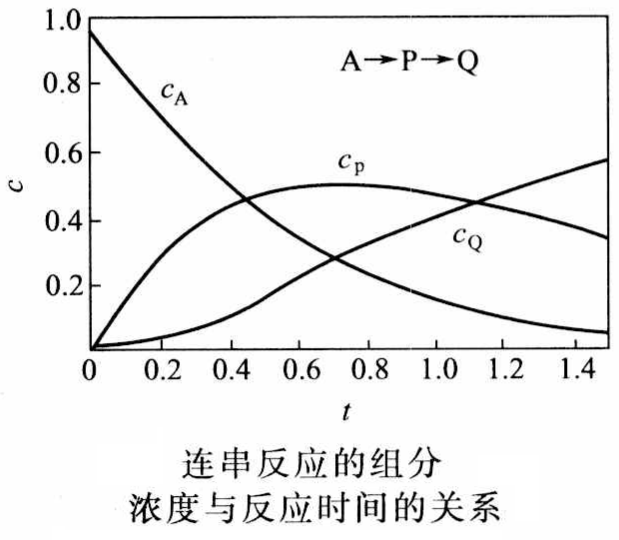
\includegraphics[width=4.5cm]{figs/fig3.3.png}
    \end{columns}
    
\end{frame}


\begin{frame}{连串反应}
    当目的产物为P时，就需要控制反应时间，以使P的收率最大。
    
    将式$c_{\mathrm{P}}=\frac{k_{1} c_{\mathrm{A} 0}}{k_{1}-k_{2}}(e^{-k_{2} t}-e^{-k_{1} t})$对$t$求导，然后令$\mathrm{d}c_\mathrm{p}/\mathrm{d}t=0$可得最优反应时间
    $$t_{\mathrm{opt}}=\frac{\ln (k_{1} / k_{2})}{k_{1}-k_{2}}$$
    将$t_{\mathrm{opt}}$代回可求P的最大浓度。

    当目的产物为Q时，则反应时间越长，Q的收率越大。

    以上的讨论是针对包括两个一级反应的连串反应，其结论也可推广到更多反应时的场合，只要是中间产物，必存在极大浓度。对于非一级反应，可按上边的方法同样处理，只是大多数情况都很难获得解析解，需用数值解法。
    
    确定反应时间后，可根据式$V_\mathrm{r}=Q_0(t+t_0)$求反应体积。
\end{frame}


\begin{frame}[t]
    \frametitle{}
    \begin{block}{例\quad \scriptsize{《化学反应工程》李倩，化学工业出版社，97页例3-8}}
        等温一级不可逆连串反应$\mathrm{A} \stackrel{k_{1}}{\longrightarrow} \mathrm{P} \stackrel{k_{2}}{\longrightarrow} \mathrm{S}$在间歇釜式反应器中进行，反应物A的初始浓度为\SI{2}{mol.m^{-3}}，反应速率常数$k_1=\ $\SI{0.5}{h^{-1}}，$k_2=\ $\SI{0.25}{h^{-1}}，求A的转化率为80\%时，目的产物P的选择性。
        \tcblower
        \pause
        \[
            \begin{aligned}
                 t&=\frac{1}{k_{1}} \ln \frac{1}{1-X_{\mathrm{A}}} = \frac{1}{0.5} \ln \frac{1}{1-0.8} = 3.22 \ \mathrm{h}\\
                 c_{\mathrm{P}}&=\frac{k_{1} c_{\mathrm{A} 0}}{k_{1}-k_{2}}\left(e^{-k_{2} t}-e^{-k_{1} t}\right) = 0.9888 \ \si{mol.m^{-3}}\\
                 S_{\mathrm{P}}&=\frac{c_{\mathrm{P}}}{c_{\mathrm{A0}}X_{\mathrm{A}}} = \frac{0.9888}{0.8\times 2} = 61.8\%
            \end{aligned}
        \]
    \end{block}
\end{frame}


\begin{frame}[t]{}
    \begin{block}{例3.4}
        在间歇釜式反应器中等温下进行下列反应
        $$\mathrm{NH}_{3}+\mathrm{CH}_{3} \mathrm{OH} \stackrel{k_{1}}{\longrightarrow} \mathrm{CH}_{3} \mathrm{NH}_{2}+\mathrm{H}_{2} \mathrm{O}$$
        $$\mathrm{CH}_{3} \mathrm{NH}_{2}+\mathrm{CH}_{3} \mathrm{OH} \stackrel{k_{2}}{\longrightarrow}\left(\mathrm{CH}_{3}\right)_{2} \mathrm{NH}+\mathrm{H}_{2} \mathrm{O}$$
        这两个反应对各自的反应物均为一级，并已知反应温度下$k_2/k_1=0.68$，试计算一甲胺的最大收率和与其相应的氨转化率。
    \end{block}
\end{frame}


\section{连续釜式反应器的反应体积}


\begin{frame}{连续釜式反应器的反应体积}
    釜式反应器的物料衡算式：
    \[
        Q_0c_{i0}=Qc_{i}-\mathcal{R}_iV_\mathrm{r}+\mathrm{d}n_i/\mathrm{d}t
    \]
    实际生产中的连续釜式反应器几乎都是在定态下操作，因之各股物流以及反应器的所有参数均不随时间而变，从而不存在时间自变量。

    连续釜式反应器的物料衡算式：
    \[
        Q_0c_{i0}=Qc_{i}-\mathcal{R}_iV_\mathrm{r}
    \]
    另一方面，这类反应器多用于在液相中进行的反应，反应过程中液体体积的变化不显著，完全可以认为是在等容下进行反应。假定物料进出口的流量相等，对设计计算的精确度带来的影响极其有限，这样可简化为
    \[
        V_{\mathrm{r}}=\frac{Q_{0}\left(c_{i}-c_{i 0}\right)}{\mathcal{R}_i}
    \]
    这就是连续釜式反应器反应体积的计算公式。
\end{frame}


\begin{frame}
    \frametitle{连续釜式反应器的反应体积}

    如果反应器中只进行一个反应，并以组分A为关键组分，则

    \[
        V_{\mathrm{r}}=\frac{Q_{0}(c_{\mathrm{A} 0}-c_{\mathrm{A}})}{-\mathscr{R}_{\mathrm{A}}}=\frac{Q_{0} c_{\mathrm{A} 0} X_{\mathrm{Af}}}{-\mathscr{R}_{\mathrm{A}}(X_{\mathrm{Af}})}
    \]

    \begin{itemize}
        \item[\bullet]定态下操作的连续釜式反应器系在等温、等浓度下进行反应，因而也是在等反应速率下反应，即$\mathscr{R}_{\mathrm{A}}$在整个反应进程中均为常数，既不随空间而变，也不随时间而变。
        \item[\bullet] 通过简单的代数运算便可确定釜式反应器的反应体积。
        \item[\bullet] 等速操作是连续釜式反应器不同于其他反应器的一个显著特点。
        \item[\bullet] $\mathscr{R}_{\mathrm{A}}$应按反应器内的反应物料组成计算，由于此组成与出口物料组成相同，也可以说是按出口物料组成计算。
    \end{itemize}

\end{frame}


\begin{frame}[t]
    \frametitle{}
    \begin{question}
        在\highlight{间歇}操作的釜式反应器中进行己二酸（A）和己二醇（B）等摩尔比缩聚反应。动力学方程式为$r_\mathrm{A} = kc_\mathrm{A}^2$\ \si{kmol/(L.h)}。其中，速率常数$k = 118.2$ \ \si{L/(kmol.h)}，反应物的初始浓度$c_\mathrm{A0} = 0.005$\ \si{kmol/L}。若每天处理2400 kg己二酸，每批辅助时间为1 h，反应器装填系数为0.8，求转化率为$X_\mathrm{Af}$时所需反应器的体积。
        % \tcblower
        \begin{table}
            \centering
            \begin{tabular}{cc||cc||cc}
                \bottomrule
                $X_\mathrm{Af}$ & 反应器体积\ (\si{m^3}) & $X_\mathrm{Af}$ & 反应器体积\ (\si{m^3}) & $X_\mathrm{Af}$ & 反应器体积\ (\si{m^3}) \\ \hline
                0.1 & 0.16 & 0.5 & 0.37 & 0.9 & 2.22 \\ 
                0.2 & 0.19 & 0.6 & 0.48 & 0.99 & 23.08 \\ 
                0.3 & 0.24 & 0.7 & 0.68 & 0.999 & 231.7 \\ 
                0.4 & 0.29 & 0.8 & 1.06 & 0.9999 & 2318 \\ \toprule
            \end{tabular}
        \end{table}
    \end{question}
\end{frame}


\begin{frame}[t]
    \frametitle{}
    \begin{question}
        在\highlight{连续}操作的釜式反应器中进行己二酸（A）和己二醇（B）等摩尔比缩聚反应。动力学方程式为$r_\mathrm{A} = kc_\mathrm{A}^2$\ \si{kmol/(L.h)}。其中，速率常数$k = 118.2$ \ \si{L/(kmol.h)}，反应物的初始浓度$c_\mathrm{A0} = 0.005$\ \si{kmol/L}。若每天处理2400 kg己二酸，反应器装填系数为0.8，求转化率为$X_\mathrm{Af}$时所需反应器的体积。
        \begin{table}
            \centering
            \begin{tabular}{cc||cc}
                \bottomrule
                $X_\mathrm{Af}=0.1$ & 410\quad 411 \quad 412 & $X_\mathrm{Af}=0.7$ & 级数 \quad 奈何桥也是桥 \\ 
                $X_\mathrm{Af}=0.2$ & 421 \quad 424 \quad 425
                & $X_\mathrm{Af}=0.8$ & 压力 \quad G.T.I.大家庭  \\ 
                $X_\mathrm{Af}=0.3$ & 1 \quad 123 \quad 12138 & $X_\mathrm{Af}=0.9$ & [默认组名] \quad 没有这个组  \\ 
                $X_\mathrm{Af}=0.4$ & 227 \quad 233 \quad 241 & $X_\mathrm{Af}=0.99$ & 反应级数 \quad 哈基米典礼 \\
                $X_\mathrm{Af}=0.5$ & 413 \quad 12345 & $X_\mathrm{Af}=0.999$ & 欧内的手组 \quad 化工科技组  \\
                $X_\mathrm{Af}=0.6$ & 沉淀 \quad 新建分组 & $X_\mathrm{Af}=0.9999$ & 私人小组 \quad 没组的来  \\  \toprule
            \end{tabular}
            \vspace{-1pt}
        \end{table}
    \end{question}
\end{frame}


\begin{frame}[t]
    \frametitle{}
    \begin{question}
        在\highlight{连续}操作的釜式反应器中进行己二酸（A）和己二醇（B）等摩尔比缩聚反应。动力学方程式为$r_\mathrm{A} = kc_\mathrm{A}^2$\ \si{kmol/(L.h)}。其中，速率常数$k = 118.2$ \ \si{L/(kmol.h)}，反应物的初始浓度$c_\mathrm{A0} = 0.005$\ \si{kmol/L}。若每天处理2400 kg己二酸，每批辅助时间为1 h，求转化率为$X_\mathrm{Af}$时所需反应体积。
        % \tcblower
        \begin{table}
            \centering
            \begin{tabular}{cc||cc||cc}
                \bottomrule
                $X_\mathrm{Af}$ & 反应体积\ (\si{m^3}) & $X_\mathrm{Af}$ & 反应体积\ (\si{m^3}) & $X_\mathrm{Af}$ & 反应体积\ (\si{m^3}) \\ \hline
                0.1 & 0.286 & 0.5 & 0.464 & 0.9 & 20.86 \\ 
                0.2 & 0.724 & 0.6 & 0.869 & 0.99 & $2.3\times 10^3$ \\ 
                0.3 & 0.142 & 0.7 & 1.803 & 0.999 & $2.3\times 10^5$ \\ 
                0.4 & 0.258 & 0.8 & 4.636 & 0.9999 & $2.3\times 10^{7}$ \\ \toprule
            \end{tabular}
        \end{table}
    \end{question}
\end{frame}


\begin{frame}[t]
    \frametitle{}
    \begin{question}
        讨论：同样的物料处理量，达到同样的转化率，为什么采用连续操作所需的反应体积与间歇操作反应体积不同？
        \tcblower
        \pause
        \begin{itemize}
          \item 间歇反应器是变速操作，开始时反应速率最大，终了时最小
          \item 连续釜式反应器是等速操作，且恰恰是在相应于间歇反应器的最小反应速率下操作
          \item 间歇操作需要辅助时间
        \end{itemize}
    \end{question}
\end{frame}


\begin{frame}
    \frametitle{空时}

    间歇反应器的反应体积是通过反应时间及物料处理量来确定的。定态操作的连续釜式反应器则是由物料衡算式直接计算反应体积。为了对连续反应器的生产能力作比较，往往引用空间时间（简称空时）这一概念，其定义为
    
    \[\tau = \frac{V_\mathrm{r}}{Q_0} = \frac{\text{反应体积}}{\text{进料体积流量}}\]

    \begin{itemize}
        \item[\bullet] 空时具有时间的因次。
        \item[\bullet] 对于等容均相反应过程，空时等于物料在反应器内的平均停留时间。
        \item[\bullet] 空时越小，表示该反应器的处理物料量越大，空时大则相反。
        \item[\bullet] 若在进出口物料组成相同的条件下比较两个连续反应器，空时小者，生产能力大，当然，两者的进料体积流量必须按相同的温度及压力计算。
    \end{itemize}


\end{frame}


\begin{frame}
    \frametitle{空速}

    空时的倒数为空速，其意义是单位反应体积单位时间内所处理的物料量，因次为[时间]$^{-1}$。空速越大，反应器的生产能力越大。

    为了便于比较，通常采用标准情况下的体积流量。
    \begin{itemize}
        \item[\bullet] 对于使用固体催化剂的反应，往往以催化剂的质量多少表示反应体积的大小，因此有质量空速与体积空速之分：前者为单位质量催化剂单位时间内处理的物料量；后者则基于单位体积催化剂计算，且一般是指催化剂的堆体积。

        \item[\bullet] 有时反应进料为液体，经汽化后进行气相反应，当进料流量按液体体积计算时所得的空速，称为液空速。

        \item[\bullet] 此外还有指某一特定反应组分计算的空速，如碳空速、烃空速等。
    \end{itemize}
    使用时必须注意，不要混淆。
\end{frame}


\begin{frame}[t]
    \frametitle{}
    \begin{example}
        等温下进行某均相反应\ce{A -> B}，$r_\mathrm{A}=5.2c_\mathrm{A}$ (\si{mol.L^{-1}.h^{-1}})，每天生产B 20 kmol，A的初始浓度为2mol/L，最终转化率为80\%。
        
        (1)采用连续釜式反应器，计算所需反应体积。(2)采用间歇釜式反应器，辅助时间15min，计算所需反应体积。(3)采用连续釜式反应器，保持空时与上述间歇反应器的反应时间相同，最终转化率能否达到80\%？
        \tcblower
        \only<1>{
            
        }
    \only<2>{
        (1) 
    \[
        Q_0 = \frac{20000}{24\times 0.8 \times 2} = 520.8 \mathrm{L}
    \]
    \[
        V_{\mathrm{r}}=\frac{Q_{0} c_{\mathrm{A} 0} X_{\mathrm{A}}}{kc_{\mathrm{A0}}(1-X_{\mathrm{A}})}=  \frac{520.8 \times 0.8}{5.2 \times (1-0.8)}=401\mathrm{L}
    \]
    }
    \only<3>{
        (2)
        \[
        t =\frac{1}{k}\ln \frac{1}{(1-X_{\mathrm{A}})} =0.31 \mathrm{h}
    \]
    \[
        V_{\mathrm{r}}=Q_{0}(t+t_0)=520.8\times (0.31+0.25)=292\mathrm{L}
    \]
    }
    \only<4>{
        (3)
        \[
        V_{\mathrm{r}} = Q_{0}\tau = 520.8 \times 0.31 = 161 \mathrm{L}
    \]
    \[
        \frac{Q_{0} c_{\mathrm{A} 0} X_{\mathrm{A}}}{kc_{\mathrm{A0}}(1-X_{\mathrm{A}})} = 161  \mathrm{L}
    \]
    \[
        X_{\mathrm{A}} =61.7\%
    \]
    }
    
    \end{example}
\end{frame}


\section{连续釜式反应器的串联与并联}


\begin{frame}
    \frametitle{多釜串联的全混流反应器}

    由于反应器出口处反应物浓度最低，故全混流反应器总是在最低的反应物浓度下操作，很多情况下将会影响反应的效率。为了利用全混流反应器的混合均匀、温度易控的优点，又使反应不全部在反应物浓度最低的条件下进行，工业上经常将全混流反应器串联起来使用，称为多釜串联的全混流反应器(CSTRs in series)。

    \centering 
    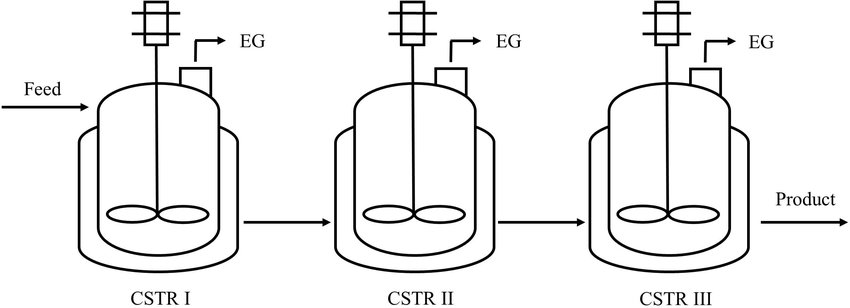
\includegraphics[height=4cm]{figs/CSTRs-in-series.png}

\end{frame}


\begin{frame}
    \frametitle{连续釜式反应器反应体积的几何图示}

    连续釜式反应器反应体积$V_{\mathrm{r}}=\frac{Q_{0} c_{\mathrm{A} 0} X_{\mathrm{A}}}{-\mathscr{R}_{\mathrm{A}}}$，以$X_{\mathrm{A}}$对$\frac{1}{-\mathscr{R}_{\mathrm{A}}}$作图，

    \begin{minipage}{0.48\linewidth}
        \begin{figure}[htpb]
            \centering
            
\includegraphics[width=.9\linewidth]{fig3.4}
        \end{figure}
    \end{minipage}\hfill
    \begin{minipage}{0.48\linewidth}
        \begin{enumerate}
          \item 单釜操作：反应体积与OADK面积成正比
          \item 两个反应器串联，反应体积与阴影部分面积成正比
          \item 串联釜数越多，总反应体积越小
        \end{enumerate}
    \end{minipage}

\end{frame}


\begin{frame}
    \frametitle{多釜并联}
    若为反常动力学，则应各釜单独操作，即采用并联方式。
    \begin{minipage}{0.48\linewidth}
        \begin{figure}[htpb]
            \centering
            
\includegraphics[width=.9\linewidth]{fig3.4b}
        \end{figure}
    \end{minipage}\hfill
    \begin{minipage}{0.48\linewidth}
        \begin{figure}[htpb]
            \centering
            
\includegraphics[width=.9\linewidth]{fig3.5}
        \end{figure}
    \end{minipage}
\end{frame}


\begin{frame}
    \frametitle{串联釜式反应器的计算：已知反应器体积计算最终转化率}

    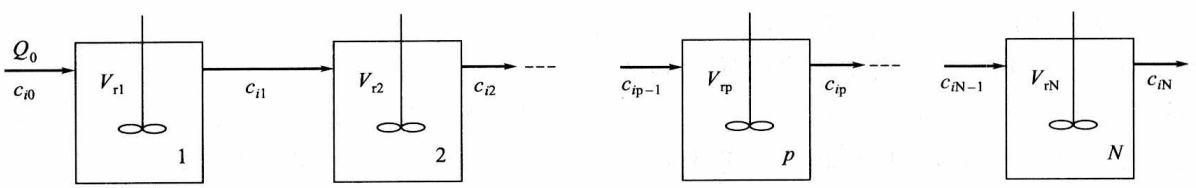
\includegraphics[width=\linewidth]{figs/fig3.6.png}

    由$N$个反应体积分布为，$V_\mathrm{r1}$，$V_\mathrm{r2}$，$\cdots$，$V_{\mathrm{r}N}$的釜组成的串联釜式反应器。若求最终转化率或收率，对各釜分别作关键组分$i$的物料衡算得下列方程组
    \[
        V_{\mathrm{rp}}=\frac{Q_{0}(c_{i \mathrm{p-1}}-c_{i \mathrm{p}})}{-\mathcal{R}_{i\mathrm{p}}} \qquad\left[\begin{array}{l}
        p=1,2, \cdots, N \\
        i=1,2, \cdots, K 
        \end{array}\right]
    \]

    计算从第1釜开始，由于该釜的进口组成已知，可求出口组成，这也就是第2釜的进口组成。依此类推，直至第N釜即为所求。这种算法称为\highlight{逐釜计算法}。

\end{frame}


\begin{frame}[t]
    \frametitle{}
    \begin{example}
        采用两个体积均为200 L的连续釜式反应器串联，等温下进行某均相反应\ce{A -> B}，$r_\mathrm{A}=5.2c_\mathrm{A}$ (\si{mol.L^{-1}.h^{-1}})，进料体积流量为520.8 L/h，A的初始浓度为2 mol/L，计算最终转化率。
        \tcblower
    \pause
    
    \begin{minipage}{0.48\linewidth}
        计算第一釜出口转化率：
        \[
        \begin{aligned}
            V_{\mathrm{r}}&=\frac{Q_{0} c_{\mathrm{A} 0} X_{\mathrm{A1}}}{kc_{\mathrm{A0}}(1-X_{\mathrm{A1}})} \\
            200 &= \frac{520.8X_{\mathrm{A1}}}{5.2\times(1-X_{\mathrm{A1}})} \\
            X_{\mathrm{A1}} &= 66.632\%
        \end{aligned}
        \]
    \end{minipage}\hfill
    \begin{minipage}{0.48\linewidth}
        计算第二釜出口转化率：
        \[
        \begin{aligned}
            V_{\mathrm{r}}&=\frac{Q_{0} c_{\mathrm{A} 0} (X_{\mathrm{A2}}-X_{\mathrm{A1}})}{kc_{\mathrm{A0}}(1-X_{\mathrm{A2}})} \\
            200 &= \frac{520.8(X_{\mathrm{A2}}-0.66632)}{5.2\times(1-X_{\mathrm{A2}})} \\
            X_{\mathrm{A2}} &= 88.866\%
        \end{aligned}
        \]
    \end{minipage}
    
    与单个400L反应器连续操作相比，双200L釜串联能达到更高转化率。
    \end{example}
\end{frame}


\begin{frame}
    \frametitle{釜数和各釜的体积的确定}

    \large 实际设计中往往是已知进料量和组成，确定达到规定的输出物料组成时所需的釜数和各釜的反应体积。

    \begin{enumerate}
      \item 一般情况下，釜数越多，总反应体积越小，从这点看，多用几个釜串联操作是有利的。
      \item 但是，釜数多了，相应地管道阀门和控制仪表等也要增多，操作的复杂程度也随之增加，所以，应根据具体情况从经济的角度出发确定最佳的釜数。
      \item 此外，各釜的操作温度及浓度的确定，即各釜的反应体积间的比例是一个优化问题。
      \item 一般把各釜做成相同的大小，是从机械加工制造方便的角度出发的。
    \end{enumerate}
\end{frame}


\begin{frame}
    \frametitle{串联釜式反应器的计算(一级单一反应)}

    以一级单一反应为例，以反应物A为关键组分
    \[
        V_{\mathrm{rp}}=\frac{Q_{0}(c_{\mathrm{Ap}-1}-c_{\mathrm{Ap}})}{(-\mathscr{R}_{\mathrm{Ap}})} =\frac{Q_{0} c_{\mathrm{A} 0}(X_{\mathrm{Ap}}-X_{\mathrm{Ap}-1})}{-\mathscr{R}_{\mathrm{Ap}}(X_{\mathrm{Ap}})} =\frac{Q_{0}(X_{\mathrm{Ap}}-X_{\mathrm{Ap}-1})}{k(1-X_{\mathrm{Ap}})}
    \]

    假定各釜反应体积相等，则各釜的空时相等，设为$\tau$；各釜温度相同，反应速率常数均为$k$。则上式可变为
    \[
        \frac{1-X_{\mathrm{Ap}-1}}{1-X_{\mathrm{Ap}}}=1+k \tau \qquad (p=1,2,\cdots , N)
    \]

    将这$N$个方程相乘则有
    \[
        \frac{1}{1-X_{\mathrm{AN}}}=(1+k \tau)^{N} \quad \text{或} \quad \tau=\frac{1}{k}\left[\left(\frac{1}{1-X_{\mathrm{AN}}}\right)^{1 / N}-1\right]
    \]

\end{frame}


\begin{frame}[t]{}
    \begin{example}
        采用双釜串联的连续釜式反应器，等温下进行某均相反应\ce{A -> B}，$r_\mathrm{A}=5.2c_\mathrm{A}$ (\si{mol.L^{-1}.h^{-1}})，每天生产B 20 kmol，A的初始浓度为2 mol/L，最终转化率为80\%。计算总反应体积。
    \tcblower
    \pause
    \[
        \tau=\frac{1}{5.2}\left[\left(\frac{1}{1-0.8}\right)^{1 / 2}-1\right]=0.2377 \mathrm{h}
    \]

    \[
        V_\mathrm{r}=2Q_0 \tau = 2 \times 520.8 \times 0.2377 = 247.59 \mathrm{L}
    \]
    \end{example}
\end{frame}


\begin{frame}
    \frametitle{作图法求串联釜式反应器出口转化率}

    \begin{columns}[c]
        \column{5cm}
            \\~
            \\~
            \\    
            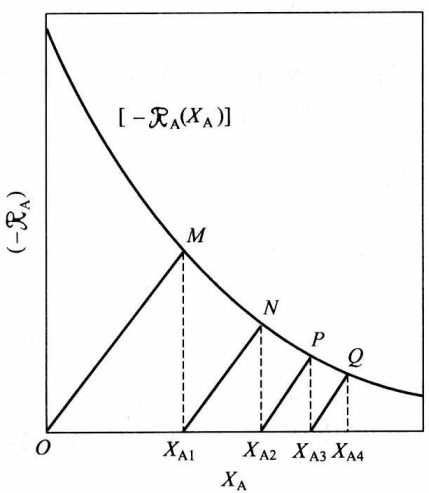
\includegraphics[width=\linewidth]{figs/fig3.7.png}
        \column{8.5cm}
            对于非一级反应，需要逐釜计算。

            将$V_{\mathrm{rp}}=\frac{Q_{0} c_{\mathrm{A} 0}(X_{\mathrm{Ap}}-X_{\mathrm{Ap}-1})}{-\mathscr{R}_{\mathrm{Ap}}(X_{\mathrm{Ap}})}$改写成
            \[
                -\mathscr{R}_{\mathrm{A}}=\frac{c_{\mathrm{A} 0}}{\tau_{\mathrm{p}}} X_{\mathrm{Ap}}-\frac{c_{\mathrm{A} 0}}{\tau_{\mathrm{p}}} X_{\mathrm{Ap}-1}
            \]

            在$X_\mathrm{A}$-$(-\mathcal{R}_\mathrm{A})$图上，物料衡算式为一直线，其斜率为$c_{\mathrm{A} 0} / \tau_{\mathrm{p}}$。
            
            各釜温度相图，所以只需根据反应速率方程绘制一条动力学曲线。因为出口转化率既要满足反应速率方程，又要符合物料衡算式，所以可由两者交点决定釜的出口状态。
    \end{columns}

\end{frame}


\begin{frame}
    \frametitle{二级反应$-\mathscr{R}_{\mathrm{A}}=kc_\mathrm{A}^2$函数图像长什么样}
    \begin{figure}[htpb]
        \centering
        
\includegraphics[width=.8\linewidth]{函数图像1}
    \end{figure}
\end{frame}


\begin{frame}
    \frametitle{二级反应$-\mathscr{R}_{\mathrm{A}}=kc_\mathrm{A}^2$在转化率[0, 1]的函数图像}
    \begin{figure}[htpb]
        \centering
        
\includegraphics[width=.8\linewidth]{函数图像2}
    \end{figure}
\end{frame}


\begin{frame}[t]{}
    \begin{redblock}{作图法计算}
        等温下进行某均相反应\ce{A -> B}，$r_\mathrm{A}=5.2c_\mathrm{A}^2$ (\si{mol.L^{-1}.h^{-1}})，每天生产B 20 kmol，A的初始浓度为2 mol/L，最终转化率为80\%。采用三个等体积反应釜串联，计算总反应体积。
    \tcblower
    \end{redblock}
\end{frame}


\begin{frame}
    \frametitle{串联釜式反应器各釜最佳反应体积比}

    釜数及最终转化率已规定的情况下，为了使总的反应体积最小，各釜的反应体积存在一最佳的比例。现设所进行的为单一反应，则总反应体积
    \[
        V_{\mathrm{r}}=V_{\mathrm{r} 1}+\cdots+V_{\mathrm{rN}}=Q_{0} c_{\mathrm{A} 0}\left[\frac{X_{\mathrm{A} 1}-X_{\mathrm{A} 0}}{\left(-\mathscr{R}_{\mathrm{A} 1}\right)}+\frac{X_{\mathrm{A} 2}-X_{\mathrm{A} 1}}{\left(-\mathscr{R}_{\mathrm{A} 2}\right)}+\cdots+\frac{X_{\mathrm{AN}}-X_{\mathrm{AN}-1}}{\left(-\mathscr{R}_{\mathrm{AN}}\right)}\right]
    \]

    将上式分别对$X_\mathrm{Ap}$求导得
    \[
        \frac{\partial V_{\mathrm{r}}}{\partial X_{\mathrm{Ap}}}=Q_{0} c_{\mathrm{A} 0}\left[\frac{1}{\left(-\mathscr{R}_{\mathrm{Ap}}\right)}-\frac{1}{\left(-\mathscr{R}_{\mathrm{Ap}+1}\right)}+\left(X_{\mathrm{Ap}}-X_{\mathrm{Ap}-1}\right) \frac{\partial \frac{1}{\left(-\mathscr{R}_{\mathrm{Ap}}\right)}}{\partial X_{\mathrm{Ap}}}\right]
    \]
    令${\partial V_{\mathrm{r}}}/{\partial X_{\mathrm{Ap}}}=0$有$\frac{1}{\left(-\mathscr{R}_{\mathrm{Ap}+1}\right)}-\frac{1}{\left(-\mathscr{R}_{\mathrm{Ap}}\right)}=\left(X_{\mathrm{Ap}}-X_{\mathrm{Ap}-1}\right) \frac{\partial \frac{1}{\left(-\mathscr{R}_{\mathrm{Ap}}\right)}}{\partial X_{\mathrm{Ap}}}$
    
    这就是保证总反应体积最小所必须遵循的条件。解方程式组可得$X_{\mathrm{Ap}}$和$V_{\mathrm{rp}}$。
    
\end{frame}


\begin{frame}
    \frametitle{串联釜式反应器各釜最佳反应体积比}

    进行一级不可逆反应时，将$(-\mathscr{R}_\mathrm{A})=k c_{\mathrm{A} 0}(1-X_\mathrm{A})$代入上式，化简得：
    \[
        \frac{X_{\mathrm{Ap}+1}-X_{\mathrm{Ap}}}{1-X_{\mathrm{Ap}+1}}=\frac{X_{\mathrm{Ap}}-X_{\mathrm{Ap}-1}}{1-X_{\mathrm{Ap}}}
    \]
    上式可改写成
    \[
        \frac{Q_{0} c_{\mathrm{A} 0}(X_{\mathrm{Ap}+1}-X_{\mathrm{Ap}})}{k c_{\mathrm{A} 0}(1-X_{\mathrm{Ap}+1})}=\frac{Q_{0} c_{\mathrm{A} 0}(X_{\mathrm{Ap}}-X_{\mathrm{Ap}-1})}{k c_{\mathrm{A} 0}(1-X_{\mathrm{Ap}})}
    \]
    即\[V_{\mathrm{rp}+1}=V_{\mathrm{rp}}\]

    由此可见，串联釜式反应器进行一级不可逆反应时，各釜的反应体积相等时，总反应体积最小。

\end{frame}


\begin{frame}
    \frametitle{串联釜式反应器各釜最佳反应体积比}

    用串联釜式反应器进行$\alpha$ 级反应时，最佳反应体积：
    \begin{itemize}
        \item[1] $\alpha=1$时，各釜体积相等
        \item[2] $\alpha>1$时，小釜在前，大釜在后
        \item[3] $\alpha<1$时，大釜在前，小釜在后
        \item[4] $\alpha=0$时，反应速率与浓度无关，无论多少釜串联，与单釜反应体积相等
        \item[5] $\alpha<0$时，单釜操作优于串联操作
    \end{itemize}

\end{frame}


\begin{frame}[t]{}
    \begin{example}
        以硫酸为催化剂，由醋酸和丁醇反应可制得醋酸丁酯。仓库里闲置着两台反应釜，一台的反应体积为\SI{3}{m^3}，另一台则为\SI{1}{m^3}。现拟将它们用来生产醋酸丁酯，初步决定采用等温连续操作，原料中醋酸的浓度为\SI{0.15}{kmol.m^3}，丁醇则大量过剩，该反应对醋酸为2级，在反应温度下反应速率常数为\SI{1.2}{L.mol^{-1}.h^{-1}}，要求醋酸的最终转化率不小于50\%。
        
        (1) 你认为采用怎样的连接方式醋酸丁酯的产量最大？为什么？试计算你所选用的方案得到的醋酸丁酯产量。
        
        (2) 如果进行的反应是一级反应，这两台反应器的串联方式又应如何？

        (3)如果进行的反应是一级反应，并更换为两台反应体积均为\SI{2}{m^3}的反应器串联，醋酸丁酯产量是多少？
    \end{example}

\end{frame}


\section{釜式反应器中复合反应的收率与选择性}


\begin{frame}
    \frametitle{复合反应的收率与选择性的影响因素}

    \large 在反应器中进行复合反应时，目的产物的收率如何，是首先要考虑的事，因为它直接影响到产品的数量与质量；反应选择性也同样重要，它反映了原料利用的程度。
    
    \begin{itemize}
        \item[\bullet] 反应器的型式
        \item[\bullet] 反应器的操作方式
        \item[\bullet] 反应器的操作条件
    \end{itemize}
    下面将针对釜式反应器对这些影响因素进行分析讨论。

\end{frame}


\begin{frame}
    \frametitle{总收率与总选择性}

    设生成lmol目的产物P所需反应物A的量为$\mu_\mathrm{PA}$ mol，由第二章知，瞬时选择性为
    \[
        S=\mu_{\mathrm{PA}} \frac{\mathscr{R}_{\mathrm{p}}}{(-\mathscr{R}_{\mathrm{A}})}=\mu_{\mathrm{PA}} \frac{\mathrm{d} n_{\mathrm{p}}}{(-\mathrm{d} n_{\mathrm{A}})}=\frac{\mathrm{d} Y_{\mathrm{p}}}{\mathrm{d} X_{\mathrm{A}}}
    \]
    由于$S$为瞬时值，显然$X_\mathrm{A}$和$Y_\mathrm{P}$也都是瞬时值。就间歇反应器而言三者均随时间而变；而对于定态下操作的流动反应器，三者均随位置而改变（连续釜式反应器例外）。如果将上式改写成$\mathrm{d}Y_\mathrm{P}=S\mathrm{d}X_\mathrm{A}$并积分之得
    \[
        Y_{\mathrm{Pf}}=\int_{0}^{X_{\mathrm{Af}}} S \mathrm{~d} X_{\mathrm{A}}
    \]
    此时$Y_{\mathrm{Pf}}$称为总收率或最终收率，$X_{\mathrm{Af}}$为总转化率或最终转化率，两者不再是瞬时值，而是反应过程的总结果，即$Y_{\mathrm{Pf}}$和$X_{\mathrm{Af}}$系对整个反应器而言的值。
\end{frame}


\begin{frame}
    \frametitle{总收率与总选择性}

    由转化率、收率和选择性的定义得
    \[
        Y_{\mathrm{Pf}}=S_\mathrm{O}X_{\mathrm{Af}}
    \]
    $S_\mathrm{O}$叫做总选择性，是就整个反应器而言的选择性，是一个积分值，所以又叫做积分选择性。

    总选择性与瞬时选择性的关系为
    \[
        S_\mathrm{O}=\frac{1}{X_{\mathrm{Af}}}\int_0^{X_{\mathrm{Af}}}S\mathrm{d}X_{\mathrm{A}}
    \]
    总选择性与转化率的关系取决于反应动力学、反应器型式和操作方式等，一般为一个很复杂的关系式。所以，同样是釜式反应器，由于操作方式不同，虽然最终转化率一样，但最终收率却是不一样的。

\end{frame}


\begin{frame}
    \frametitle{釜式反应器的最终收率}
    \begin{figure}[htpb]
        \centering
        
\includegraphics[width=.9\linewidth]{fig3.9}
    \end{figure}
    \pause
    (a)情况，相同最终转化率下，收率大小：间歇釜>多釜串联>单个连续釜

    (b)情况，相同最终转化率下，收率大小：间歇釜<多釜串联<单个连续釜
\end{frame}


\begin{frame}{浓度对平行反应瞬时选择性的影响(第2章)}
	$$S=\frac{k_1c_\mathrm{A}^\alpha}{k_1c_\mathrm{A}^\alpha+|{\nu_\mathrm{A}}|k_2c_\mathrm{A}^\beta}=\frac{1}{1+\frac{k_2}{k_1}|{\nu_\mathrm{A}}|c_\mathrm{A}^{\beta -\alpha}}$$
	\\若温度一定，则$k_1$和$k_2$为常数，反应物浓度$c_\mathrm{A}$改变时，瞬时选择性的变化与主副反应级数有关。
	\begin{itemize}
		\item[\bullet ]  当$\alpha = \beta$时，S与浓度无关，仅为温度的函数
		\item[\bullet ]  当$\alpha > \beta$时，反应物浓度提高，S增加，高浓度操作有利
		\item[\bullet ]  当$\alpha < \beta$时，反应物浓度提高，S减小，低浓度操作有利
	\end{itemize}
\end{frame}


\begin{frame}
    \frametitle{平行反应}

    设在釜式反应器中进行如下平行反应
    \[
        \mathrm{A}+\mathrm{B} \longrightarrow \mathrm{P} \qquad r_{\mathrm{p}}=k_{1} c_{\mathrm{A}}^{\alpha_{1}} c_{\mathrm{B}}^{\beta_{1}} 
    \]
    \[
        \mathrm{~A}+\mathrm{B} \longrightarrow \mathrm{Q} \qquad r_{\mathrm{Q}}=k_{2} c_{\mathrm{A}}^{\alpha_{2}} c_{\mathrm{B}}^{\beta_{2}}
    \]    
    目的产物为P，瞬时选择性为
    \[
        S=\frac{1}{1+\frac{k_{2}}{k_{1}} c_{\mathrm{A}}^{\alpha_{2}-\alpha_{1}} c_{\mathrm{B}}^{\beta_{2}-\beta_{1}}}
    \]
    由此可见反应物系的浓度和温度是影响瞬时选择性的直接因素。比较主、副反应的反应级数，便可判定是在高浓度下操作还是在低浓度下操作有利，抑或是一个反应物浓度高而另一个低更为有利。温度条件则看主、副反应活化能的相对大小。设计反应器时就应尽可能满足这些有利的浓度和温度条件，以获得较好的产品收率。

\end{frame}


\begin{frame}
    \frametitle{釜式反应器的操作方式与加料方式}
    \begin{figure}[htpb]
        \centering
        
\includegraphics[width=.9\linewidth]{加料方式}
    \end{figure}
\end{frame}


\begin{frame}
    \frametitle{釜式反应器的操作方式与加料方式}
    \begin{figure}[htpb]
        \centering
        
\includegraphics[width=\linewidth]{fig3.10abc}
    \end{figure}
    \begin{itemize}
        \item[(a)] 如要求A和B的浓度都高，采用间歇操作是有利的
        \item[(b)] 如采用连续操作，则多釜串联为好，且组分A及B均从第一釜同时加入
        \item[(c)] 如采用不等体积的釜串联，体积依次增大会好些，因为这可使前两釜在更高一点的浓度下操作
    \end{itemize}
\end{frame}


\begin{frame}
    \frametitle{釜式反应器的操作方式与加料方式}
    $$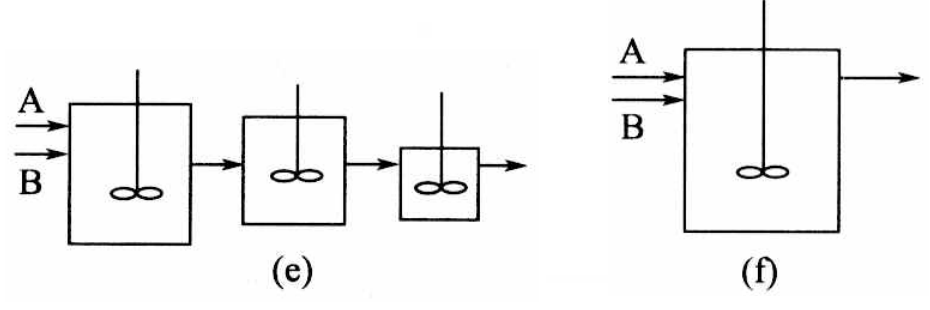
\includegraphics[width=0.8\linewidth]{figs/fig3.10ef.png}$$
    \begin{itemize}
        \item[(f)] 如要求A和B的浓度都低，采用单釜连续操作有利
        \item[(e)] 如采用多釜串联，则应做成不等体积的釜，且各釜体积依次减小，这样经过第一釜后反应物的浓度就可降得很低。
    \end{itemize}
\end{frame}


\begin{frame}
    \frametitle{釜式反应器的操作方式与加料方式}

    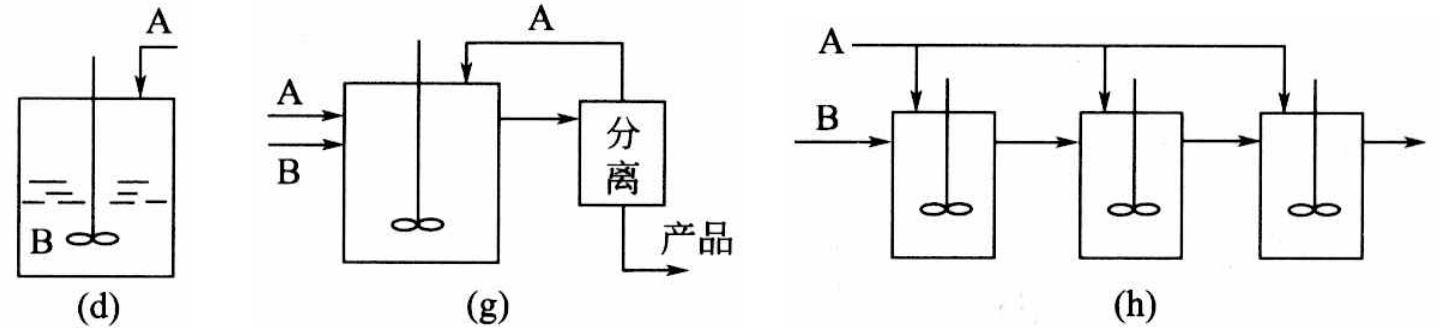
\includegraphics[width=\linewidth]{figs/fig3.10dgh.png}

    若要求一个组分浓度高另一组分浓度低，(d)(g)(h)均可选用。

    \begin{itemize}
        \item[(d)]  半间歇操作，B全部加入反应器内，A连续加入，加入速率一般由快变慢，这样可始终保持在A浓度低的情况下操作，而B的浓度则相对较大。
        \item[(h)]  连续操作，A分釜加入，结果可使A的浓度相应降低，而B的浓度则较高。
        \item[(g)] A过量配料，反应后产品分离，A和少量的B循环使用。A保持高浓度。
    \end{itemize}

\end{frame}


\begin{frame}{温度对平行反应瞬时选择性的影响（第2章）}
	设主副反应的活化能分别为$E_1$和$E_2$，且反应速率常数$k_1$和$k_2$与温度的关系符合阿伦尼乌斯公式，则
    \[
        S=\frac{1}{1+\frac{A_2}{A_1}\exp(\frac{E_1-E_2}{RT})|{\nu_\mathrm{A}}|c_\mathrm{A}^{\beta -\alpha}}
    \]
	当浓度一定时，温度对瞬时选择性的影响取决于主副反应活化能的相对大小。
	\begin{itemize}
		\item 当$E_1> E_2$时，温度越高，反应的瞬时选择性越大
		\item 当$E_2> E_1$时，温度升高，反应的瞬时选择性降低
	\end{itemize}
	\begin{alertblock}{}
        当$E_2> E_1$时，低温下瞬时选择性高，但高温下反应速率快，所以这种情况存在一最佳温度，在此温度下操作可使目的产物的产量最大。
    \end{alertblock}
\end{frame}


\begin{frame}[t]
    \frametitle{}
    \begin{block}{例3.9}
        以纯A为原料在连续釜式反应器中生产产物P，反应为
        \[
            \ch{A -> P} \qquad r_\mathrm{P} = k_1c_\mathrm{A}
        \]
        \[
            \ch{A -> U} \qquad r_\mathrm{U} = k_2c_\mathrm{A}
        \]
        反应速率常数$k_1$及$k_2$与温度的关系符合阿仑尼乌斯方程，指前因子$A_2 = 3.533\times 10^{18}$\ h$^{-1}$，$A_1 = 4.368\times 10^{15}$\ h$^{-1}$，反应活化能$E_1 = 41800$\ \si{J.mol^{-1}.K^{-1}}，$E_2 = 141000$\ \si{J.mol^{-1}.K^{-1}}。若空时为1 h，试问在什么温度下操作P的收率最大？
    \end{block}
\end{frame}


\begin{frame}[t]
    \frametitle{}
    \begin{block}{例3.9}
        解得P的收率和温度的关系如下图所示。
        \begin{figure}[htpb]
            \centering
            
\includegraphics[width=\linewidth]{例3.9}
        \end{figure}
    \end{block}
\end{frame}


% \begin{frame}
%     \frametitle{}
%     \begin{question}
%         在例3.9中，解得P的收率和温度的关系如下图所示。当T = 173 K时，$Y_\mathrm{p} = 0.999$。你认为该反应在什么温度下进行生产比较合适？        
%     \end{question}
%     \vspace{-5pt}
%     \begin{figure}[htpb]
%         \centering
%         
\includegraphics[width=.75\linewidth]{例3.9}
%     \end{figure}
% \end{frame}


\begin{frame}
    \frametitle{连串反应(间歇釜)}
    在间歇釜式反应器中进行一级不可逆连串反应：$\mathrm{A} \stackrel{k_{1}}{\longrightarrow} \mathrm{P} \stackrel{k_{2}}{\longrightarrow} \mathrm{Q}$，
    在第3节已求得
    \[
        c_{\mathrm{P}}=\frac{k_{1} c_{\mathrm{A} 0}}{k_{1}-k_{2}}\left(e^{-k_{2} t}-e^{-k_{1} t}\right) \qquad (k_1 \neq k_2)
    \]
    \[
        c_{\mathrm{P}}=c_{\mathrm{A} 0}k_1te^{-k_1t} \qquad \qquad \qquad \qquad(k_1 = k_2)
    \]
    P的最大收率
    \[
        (Y_{\mathrm{P}, \mathrm{B}})_{\max }=(k_1/k_2)^{k_2/{(k_2-k_1)}} \qquad (k_1 \neq k_2)
    \]
    \[
        (Y_{\mathrm{P}, \mathrm{B}})_{\max }=1/e=0.368 \qquad \qquad (k_1 = k_2)
    \]
    将$t=\frac{1}{k_1}\ln \frac{1}{1-X_\mathrm{A}}$代入$c_{\mathrm{P}}$表达式得转化率与收率的关系
    \[
        Y_{\mathrm{P}, \mathrm{B}}=\frac{k_{1}}{k_{1}-k_{2}}\left[(1-X_{\mathrm{A}})^{k_{2} / k_{1}}-(1-X_{\mathrm{A}})\right] \qquad (k_{1} \neq k_{2})
    \]
    \[
        Y_{\mathrm{P}, \mathrm{B}}=(X_\mathrm{A}-1)\ln (1-X_\mathrm{A}) \qquad \qquad \qquad \qquad  (k_{1} = k_{2})
    \]
\end{frame}


\begin{frame}
    \frametitle{连串反应(连续釜)}
    在连续釜式反应器中进行一级不可逆连串反应
    \[
        \mathrm{A} \stackrel{k_{1}}{\longrightarrow} \mathrm{P} \stackrel{k_{2}}{\longrightarrow} \mathrm{Q}
    \]
    A及P的物料衡算式分别为：
    \[
        V_{r}=\frac{Q_{0}(c_\mathrm{A0}-c_\mathrm{A})}{k_{1}c_\mathrm{A}}
    \]
    \[
        V_{\mathrm{r}}=\frac{Q_{0}c_{\mathrm{p}}}{k_{1}c_{\mathrm{A}}-k_{2}c_{\mathrm{p}}}
    \]
    解得
    \[
        \begin{aligned}
            c_{\mathrm{A}}&=c_{\mathrm{A}0}/(1+k_{1}\tau) \\
            c_\mathrm{P}&= \frac{k_1\tau c_{\mathrm{A}0}}{(1+k_1\tau)(1+k_2\tau)}
        \end{aligned}
    \]
\end{frame}


\begin{frame}
    \frametitle{连串反应(连续釜)}
    \vspace{-6pt}
    \[
        Y_\mathrm{P,M} = \frac{c_\mathrm{P}}{c_\mathrm{A0}}= \frac{k_1\tau}{(1+k_1\tau)(1+k_2\tau)}
    \]
    对$\tau$求导，并令$\dif Y_\mathrm{p}/\dif t = 0$，得最佳空时
    \[
        \tau_\mathrm{op} = \frac{1}{\sqrt{k_1k_2}}
    \]
    代回$Y_\mathrm{P,M}$表达式得P的最大收率
    \[
       (Y_{\mathrm{P}, \mathrm{M}})_{\max }=\frac{k_{1}}{(\sqrt{k_{1}}+\sqrt{k_{2}})^{2}}
    \]
    将$\tau = \frac{X_\mathrm{A}}{k_1(1-X_\mathrm{A})}$代入$Y_\mathrm{P,M}$表达式得转化率与收率的关系
    \[
        Y_{\mathrm{P}, \mathrm{M}}=\frac{k_{1} X_{\mathrm{A}}(1-X_{\mathrm{A}})}{k_{2} X_{\mathrm{A}}+k_{1}(1-X_{\mathrm{A}})}
    \]
\end{frame}


\begin{frame}
    \frametitle{连续釜和间歇釜的收率与转化率的比较}

    \begin{minipage}{0.48\linewidth}
        \begin{figure}[htpb]
            \centering
            
\includegraphics[width=\linewidth]{fig3.11}
        \end{figure}
    \end{minipage}\hfill
    \begin{minipage}{0.48\linewidth}
        \begin{question}
            观察图像，你能得到哪些结论？
        \end{question}
    \end{minipage}
\end{frame}


\begin{frame}
    \frametitle{连续釜和间歇釜的收率与转化率的比较}

    \begin{minipage}{0.48\linewidth}
        \begin{figure}[htpb]
            \centering
            
\includegraphics[width=\linewidth]{fig3.11}
        \end{figure}
    \end{minipage}\hfill
    \begin{minipage}{0.48\linewidth}
        \begin{itemize}
            \item 无论$k_2/k_1$为何值，相同转化率下，间歇釜式反应器P的最大收率总是大于连续釜
            \item $k_2/k_1$值越小，$Y_\mathrm{p}$差异越大
            \item 每一曲线都存在极大值
            \item ABC、DEF分别为间歇釜和连续釜最大收率的轨迹
            \item 收率总是随着$k_2/k_1$的减小而增大
        \end{itemize}
        \begin{question}
            如何减小$k_2/k_1$以得到更高收率？
        \end{question}
    \end{minipage}
\end{frame}


\begin{frame}
    \frametitle{如何减小$k_2/k_1$？}
    \begin{enumerate}
      \item 选择适宜的操作温度
        \[
        \frac{k_2}{k_1}=\frac{A_2}{A_1}\exp\bigl(\frac{E_1-E_2}{RT}\bigr)
        \]
    \begin{itemize}
      \item 若 $E_1 > E_2$ ， 温度越高 ， 则比值 ${k_2}/{k_1}$ 越小 ， 因而收率越大 ；
      \item 若 $E_1 < E_2$ ， 温度越低 ， 则比值 ${k_2}/{k_1}$ 越小 ， 因而收率越大。
      \item 温度低必然导致反应速率下降，从而反应器的生产强度减小，所以要选择适宜的操作温度
      \item 若 $E_1 = E_2$， 温度的变化已不能改变${k_2}/{k_1}$ 值 ， 但实际上仍以采用较高的温度操作为佳。
    \end{itemize}
      \item 选择合适的催化剂
        \begin{itemize}
          \item 选择有利 P 的生成反应而不利 P 的转化反应的催化剂
        \end{itemize}
    \end{enumerate}
    
\end{frame}


\begin{frame}[t]
    \frametitle{}

    \begin{example}
        原料以0.5 \si{m^3/min}的流量连续通入反应体积为20\si{m^3}的全混流反应器，进行液相反应：
        \[
        \mathrm{A} \longrightarrow \mathrm{R} \qquad r_{\mathrm{A}}=k_{1} c_{\mathrm{A}}
        \]
        \[
        \mathrm{2R} \longrightarrow \mathrm{D} \qquad r_{\mathrm{D}}=k_{2} c_{\mathrm{R}}^2
        \]    
        原料中A的浓度等于\SI{0.1}{kmol/m^3}，反应温度下，$k_1=0·1$\si{min^{-1}}，$k_2=1.25$\si{L.mol^{-1}.min^{-1}}，试计算反应器出口处A的转化率及R的收率。
    \end{example}\pause
    \begin{columns}[c]
        \column{7.5cm}
        \large $\begin{array}{l}
        \frac{V_{r}}{Q_{0}}=\frac{C_{A 0} X_{A}}{k_{1} C_{A 0}(1-X_{A})}=\frac{X_{A}}{0.1(1-X_{A})}\\
    
        X_{A}=0.80\\
        
        C_{A}=C_{A 0}(1-X_{A})=0.02  \mathrm{kmol} / \mathrm{m}^{3}  
    \end{array}$
        \column{6cm}
        \large $\begin{array}{l}
            \frac{V_{r}}{Q_{0}}=\frac{C_{R}}{k_{1} C_{A}-2 k_{2} C_{R}^{2}}\\
        
            C_{R}= \SI{0.02372}{kmol/m^3}\\
        
            Y_{R}={C_{R}}/{C_{A 0}}=23.72\%
        \end{array}$
    \end{columns}

\end{frame}


\section{半间歇釜式反应器}


\begin{frame}
    \frametitle{半间歇操作的适用场合}

    \large \begin{itemize}
        \item 要求一种反应物的浓度高而另一种反应物的浓度低时，采用半间歇操作是有利的。
        \item 需要控制反应温度时，除了通过冷却介质移走热量外，还可采用半间歇操作调节加料速度以控制温度。
        \item 为了提高某些可逆反应的产品收率，可采用半间歇操作，不断移走产物，与此同时还可提高反应过程速率。
    \end{itemize}
    半间歇釜式反应器的设计方程：
    \[
        Q_0c_{i0}=Qc_{i}-\mathcal{R}_iV_\mathrm{r}+\mathrm{d}n_i/\mathrm{d}t \qquad (i=1,2,\cdots,K)
    \]
\end{frame}


\begin{frame}
    \frametitle{半间歇釜式反应器}

    设反应器内进行如下液相反应：
    \[
    \ce{A + B -> R} \qquad r_\mathrm{A}=k'c_\mathrm{A}c_\mathrm{B}
    \]
    \[
        Q_{0} c_{\mathrm{A} 0}=Q c_{\mathrm{A}}-\mathscr{R}_{\mathrm{A}} V+\frac{\mathrm{d}(V c_{\mathrm{A}})}{\mathrm{d} t} 
    \]
    式中$V$为反应器中反应混合物的体积，其值随时间而变。假定操作开始时先向反应器中注入体积为$V_0$的B，然后连续地输入A，流量为$Q_0$，浓度为$c_\mathrm{A0}$，且不连续导出物料，即
    \[
        Q_{0} c_{\mathrm{A} 0}=-\mathscr{R}_{\mathrm{A}} V+\frac{\mathrm{d}(V c_{\mathrm{A}})}{\mathrm{d} t} 
    \]
    又设B大量过剩，则该反应可按一级反应处理
    \[
        \frac{\mathrm{d}(V c_{\mathrm{A}})}{\mathrm{d} t}+k V c_{\mathrm{A}}=Q_{0} c_{\mathrm{A} 0} 
    \]
\end{frame}


\begin{frame}
    \frametitle{半间歇釜式反应器}

    \large 若为恒速加料，任意时间下反应混合物的体积
    \[
        V=V_{0}+Q_{0} t 
    \]
    结合初始条件$t=0$，$V c_{\mathrm{A}}=0$，解该一阶线性微分方程得
    \begin{columns}[c]
        \column{7cm}
        \[
        V c_{\mathrm{A}}=\frac{Q_{0} c_{\mathrm{A} 0}}{k}[1-\exp (-k t)] 
    \]
    \[
        \frac{c_{\mathrm{A}}}{c_{\mathrm{A} 0}}=\frac{1-\exp (-k t)}{k(t+V_{0} / Q_{0})}
    \]
        \column{6.5cm}
        \[
            V c_{\mathrm{R}}=Q_{0} c_{\mathrm{A} 0} t-V c_{\mathrm{A}} 
        \]
        \[
            \frac{c_{\mathrm{R}}}{c_{\mathrm{A} 0}}=\frac{k t-[1-\exp (-k t)]}{k(t+V_{0} / Q_{0})}
        \]
    \end{columns}
    
    

\end{frame}


\begin{frame}
    \frametitle{半间歇釜式反应器}

    \begin{columns}[c]
        \column{7.8cm}
       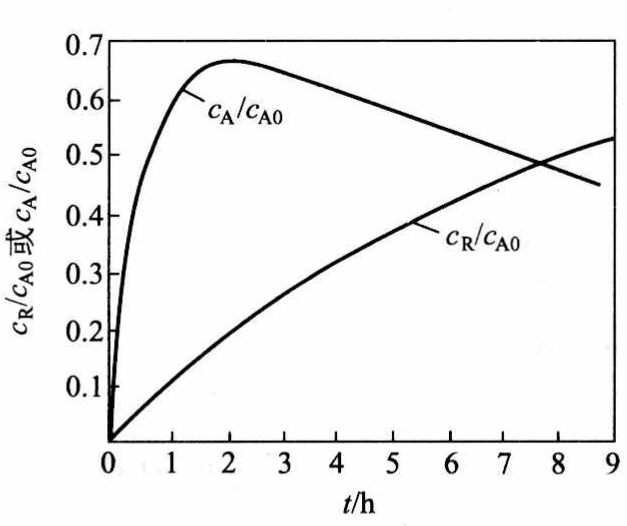
\includegraphics[width=\linewidth]{figs/fig3.12.png}
        \column{5.7cm}
        当$k=0.2\mathrm{h^{-1}}$，$V_0/Q_0=0.5\mathrm{h}$时，半间歇釜式反应器内反应组分浓度与时间的关系如图所示。
        \begin{itemize}
            \item[\bullet] 反应物A的浓度与时间的关系曲线存在一极大值
            \item[\bullet] 反应产物R的浓度总是随反应时间的增加而增加
        \end{itemize}
    \end{columns}

\end{frame}


\begin{frame}[t]
    \frametitle{}

    \begin{block}{例3.11}
        在等温间歇釜式反应器中进行下列液相反应
        \[
            \ce{A + B -> P} \qquad r_\mathrm{P}=2c_\mathrm{A} \quad \si{kmol.m^{-3}.h^{-1}}
        \]
        \[
            \ce{2A -> Q} \qquad r_\mathrm{Q}=0.5c_\mathrm{A}^2 \quad \si{kmol.m^{-3}.h^{-1}}
        \]
        先把\SI{1}{m^3}浓度为\SI{4}{kmol/m^3}的B放入釜内，然后将\SI{1}{m^3}浓度为\SI{4}{kmol/m^3}的A于\SI{3}{h}内连续均匀地加入，使之与B反应。试问A加完时，组分A和P的浓度各为多少？

    \end{block}

\end{frame}


\begin{frame}[t]
    \frametitle{}
    \begin{question}
        与例3.3相比较，在第3个小时，半间歇操作的转化率为85.57\%，低于间歇操作的99.88\%，而目的产物P的收率73\%，高于间歇操作的69.19\%。原因是什么？
    \end{question}
    \begin{figure}[htpb]
        \centering
        
\includegraphics[width=.42\linewidth]{例3-11}
    \end{figure}
\end{frame}


\section{变温间歇釜式反应器}


\begin{frame}[t]
    \frametitle{}
    \vspace{-0.4em}
    \begin{block}{企业案例：阿司匹林合成车间自动温度控制系统改造优化}
        山东新华制药二期阿司匹林合成车间存在反应器温度不稳定，热点温度过高的问题。原有西门子配套系统无法实现对温度的稳定控制，经改造优化后，实现反应工序保温阶段自动控制，控制精度提升 50\%，关键时段温度控制精度达到±0.5℃，实现稳定连续生产。
    \end{block}
    \vspace{-0.8em}
    \begin{figure}[htpb]
        \centering
        
\includegraphics[height=.3\linewidth]{新华制药}\quad 
        
\includegraphics[height=.3\linewidth]{优化控制}
    \end{figure}
\end{frame}


\begin{frame}[t]
    \frametitle{}
    \begin{redblock}{思考}
        为什么反应器保持等温有困难？
        \tcblower
        \pause
        \begin{itemize}
          \item 化学反应本身通常伴随着剧烈的热量释放或吸收
          \item 反应速率会随浓度和温度动态变化，导致生热速率波动
          \item 化学反应速率的非线性使得温度控制变得非常敏感和困难
          \item 控制系统的响应存在滞后
          \item 反应器规模越大，单位体积对应的传热面积就越小，传热能力越受限
        \end{itemize}
    \end{redblock}
\end{frame}


\begin{frame}[t]
    \frametitle{}
    \begin{redblock}{思考}
        为什么反应器保持等温有困难？
        \tcblower
        \begin{itemize}
          \item 化学反应本身通常伴随着剧烈的热量释放或吸收
          \item 反应速率会随浓度和温度动态变化，导致生热速率波动
          \item 化学反应速率的非线性使得温度控制变得非常敏感和困难
          \item 控制系统的响应存在滞后
          \item 反应器规模越大，单位体积对应的传热面积就越小，传热能力越受限
        \end{itemize}
    \end{redblock}
    \begin{alertblock}{}
        要实现等温操作需要满足什么样的条件？
    \end{alertblock}
\end{frame}


\begin{frame}
    \frametitle{反应过程能量变化}

    间歇反应过程温度与时间的关系可由能量守恒定律来确定。

    由热力学第一定律
    \[
        U = Q + W
    \]
    如果不考虑搅拌器对反应物系所作的功，则
    {\huge\[
        \dif q = \dif U
    \]}
    即反应物系与环境交换的热量等于内能的变化。
\end{frame}




\begin{frame}[t]
    \frametitle{}
    \begin{question}
        反应物系与环境交换的热量可能与哪些因素有关？如何提高反应器的换热速率？
    \tcblower
    \only<1>{
        \begin{figure}[htpb]
        \centering
        
\includegraphics[width=.3\linewidth]{夹套反应器}
    \end{figure}
    }
    \only<2>{
        \begin{figure}[htpb]
        \centering
        
\includegraphics[width=\linewidth]{冷凝器}
    \end{figure}
    }
    \only<3>{
        \begin{enumerate}
          \item 传热系数
          \item 传热面积
          \item 温差
        \end{enumerate}

    反应物系与环境交换的热量为：
    {\huge
    \[
        \dif q = UA_\mathrm{h}(T_\mathrm{c}-T)\dif t
    \]}
    式中，$U$为总传热系数；$A_\mathrm{h}$为传热面积；$T_\mathrm{c}$为环境的温度。
    }
    \end{question}
\end{frame}


\begin{frame}
    \frametitle{反应过程能量变化}
    \begin{question}
        内能变化$\dif U$如何计算？
    \end{question}
    \[
        H = U + pV
    \]
    \[
        \dif H = \dif U + \dif(pV)
    \]
    事实上反应器中物料的内能变化和焓变$\dif H$并无显著差别，特别是液相物系。
    
    所以，为了计算方便和实用的目的，用下式来代替
    \[
        \dif q = \dif U = \dif H
    \]
\end{frame}


\begin{frame}
    \frametitle{标准摩尔反应焓变的计算}
    \[
        \nu_\mathrm{A}\mathrm{A} + \nu_\mathrm{B}\mathrm{B} \longrightarrow \nu_\mathrm{P}\mathrm{P} + \nu_\mathrm{Q}\mathrm{Q}
    \]
    \[
        \Delta_\mathrm{r} H_\mathrm{m}^\ominus = \sum \nu_i \Delta_\mathrm{f}H_{m(i)}^\ominus
    \]
\end{frame}


\begin{frame}
    \frametitle{$\dif H$的计算}
        \begin{center}
        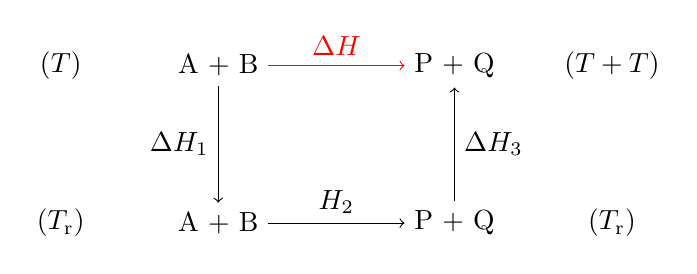
\begin{tikzpicture}
            \node (A) at (0,0) {$(T_\mathrm{r})$};
            \node (B) at (2,0) {A + B};
            \node (C) at (5,0) {P + Q};
            \node (D) at (7,0) {$(T_\mathrm{r})$};
            \node (a) at (0,2) {$(T)$};
            \node (b) at (2,2) {A + B};
            \node (c) at (5,2) {P + Q};
            \node (d) at (7,2) {$(T + \dif T)$};
            \draw [->] (b) -- (B) node[left,midway]{$\Delta H_1$};
            \draw [->] (B) -- (C) node[above,midway]{$\dif H_2$};
            \draw [->] (C) -- (c) node[right,midway]{$\Delta H_3$};
            \draw [->,red] (b) -- (c) node[above,midway]{$\Delta H$};
            \end{tikzpicture}
    \end{center}
    \[
    \begin{aligned}
        \Delta H_{1}&=m_{\mathrm{t}} \int_{T}^{T_{\mathrm{r}}} C_{\mathrm{pt}} \dif  T \approx m_{\mathrm{t}} \bar{C}_{\mathrm{pt}}(T_{\mathrm{r}}-T)  \\
        \dif  H_{2} &= \Delta H_{\mathrm{r}}\footnote{这里的$\Delta H_{\mathrm{r}}$为基于反应物A变化的反应热}(-\mathscr{R}_{\mathrm{A}}) V_{\mathrm{r}} \dif  t \\
        \Delta H_{3} &\approx m_{\mathrm{t}} \bar{C}_{\mathrm{pt}}(T+\dif  T-T_{\mathrm{r}})\\
        \dif  H &= \Delta H_{1}+\dif  H_{2}+\Delta H_{3}=m_{\mathrm{t}} \bar{C}_{\mathrm{pt}} \dif  T+\Delta H_{r}(-\mathscr{R}_{\mathrm{A}}) V_{\mathrm{r}} \dif  t 
    \end{aligned}
    \]
        
\end{frame}


\begin{frame}
    \frametitle{间歇釜式反应器的热量衡算式}
    \[
        \dif q = \dif H
    \]
    \[
        UA_\mathrm{h}(T_\mathrm{c}-T)\dif t = m_{\mathrm{t}} \bar{C}_{\mathrm{pt}} \dif  T+\Delta H_{r}(-\mathscr{R}_{\mathrm{A}}) V_{\mathrm{r}} \dif  t 
    \]
    {\huge\[
        m_{\mathrm{t}} \bar{C}_{\mathrm{pt}} \frac{\dif  T}{\mathrm{~d} t}=U A_{\mathrm{h}}(T_{\mathrm{c}}-T)-\Delta H_{\mathrm{r}} V_{\mathrm{r}}(-\mathscr{R}_{\mathrm{A}})
    \]}
    这便是间歇釜式反应器反应物料的温度与时间的关系。
\end{frame}


\begin{frame}
    \frametitle{等温间歇釜式反应器}

    若为等温过程，$\dif T=0$，则
    {\huge\[
        U A_{\mathrm{h}}(T_{\mathrm{c}}-T) = \Delta H_{\mathrm{r}}(-\mathscr{R}_{\mathrm{A}}) V_{\mathrm{r}}
    \]}
    \[
        \text{物系与环境交换的热量} = \text{反应吸收或放出的热量}
    \]
    但要做到这一点是不容易的，因为反应速率随时间而变，从而反应放热或吸热速率也随时间而变，只有物系与环境的换热速率与之相适应时，才能做到等温。所以，工业间歇反应器常是变温过程，热效应大的反应更是如此。
    对于等温间歇反应器，只根据物料衡算式以及动力学数据，便可进行设计
    \[
        n_{\mathrm{A} 0} \frac{\dif  X_{\mathrm{A}}}{\dif  t}=\left(-\mathscr{R}_{\mathrm{A}}\right) V_{\mathrm{r}}
    \]
\end{frame}


\begin{frame}
    \frametitle{变温间歇釜式反应器}
    对于变温间歇反应器，必须联立求解物料衡算式和热量衡算式，因为$\mathcal{R}_\mathrm{A}$为转化率和温度的函数
    \[
        m_{\mathrm{t}} \bar{C}_{\mathrm{pt}} \frac{\dif  T}{\mathrm{~d} t}=U A_{\mathrm{h}}(T_{\mathrm{c}}-T)-\Delta H_{\mathrm{r}} V_{\mathrm{r}}(-\mathscr{R}_{\mathrm{A}})
    \]
    和物料衡算式$n_{\mathrm{A} 0} \frac{\dif  X_{\mathrm{A}}}{\dif  t}=\left(-\mathscr{R}_{\mathrm{A}}\right) V_{\mathrm{r}}$联立后可得反应过程的温度和转化率的关系式
    {\huge\[
        m_{\mathrm{t}} \bar{C}_{\mathrm{pt}} \frac{\dif  T}{\mathrm{~d} t}=U A_{\mathrm{h}}\left(T_{\mathrm{c}}-T\right)-n_{\mathrm{A} 0} \Delta H_{\mathrm{r}} \frac{\dif  X_{\mathrm{A}}}{\dif  t}
    \]}
    可知，对一定的反应物系而言，温度与转化率的关系取决于物系与环境的换热速率。

\end{frame}


\begin{frame}
    \frametitle{绝热变温间歇釜式反应器}

    当反应在绝热条件下进行时，反应物系与环境无热交换
    {\huge\[
        m_{\mathrm{t}} \bar{C}_{\mathrm{pt}} \dif  T=n_{\mathrm{A} 0}(-\Delta H_{\mathrm{r}}) \dif  X_{\mathrm{A}}
    \]}
    若$\bar{C}_{\mathrm{pt}}$可视为常数，积分得
    {\huge\[
        T-T_{0}=\frac{n_{\mathrm{A} 0}(-\Delta H_{\mathrm{r}})}{m_{\mathrm{t}} \bar{C}_{\mathrm{pt}}} X_{\mathrm{A}}
    \]}
    $T_0$为反应开始时的温度，开始时转化率为零。$\Delta H_{\mathrm{r}}$为基准温度$T_0$下的反应热，$\bar{C}_{\mathrm{pt}}$则为$T$与$T_0$之间的平均比热容。由此可知，绝热反应过程的反应温度与转化率为线性关系。

\end{frame}


\begin{frame}
    \frametitle{研究变温操作的意义}
    \begin{itemize}
        \item 对于间歇釜式反应器要做到绝对等温是极其困难的。
        \item 对于许多化学反应，等温操作的效果不如变温操作好。
        \item 对间歇反应器而言，确定反应过程的温度与时间的关系十分必要。
        \item 温度是影响反应器操作的敏感因素，它对转化率、收率、反应速率以及反应器的生产强度都有影响。
        \item 温度不同，反应物系的物理性质也不同，从而影响到传热和传质速率及搅拌器的功率。
    \end{itemize}
\end{frame}


\begin{frame}[t]{}
    \begin{block}{例3.12}
        顺丁烯二酸酐(A)和正己醇(B)反应可生产顺丁烯二酸己酯，该反应对顺丁烯二酸酐和正己醇均为一级，反应速率常数等于
        \[
            k = 1.37 \times 10^{12} \exp{(-12628/T)} \qquad \mathrm{m^3/(kmol \cdot s)}
        \]
        现拟在间歇釜式反应器中进行该反应 ， 先将固体顺丁烯二酸酐加入釜内用蒸汽加热熔融 ， 其熔点为 326K 。 全部熔融后迅速加入己醇 ， 此液体混合物中顺丁烯二酸酐和己醇的浓度分别为\SI{4.55}{kmol/m^3}和\SI{5.34}{kmol/m^3}，该反应的反应热为\SI{-33.5}{kJ/mol}，反应混合物的$\rho \bar{C}_{p \mathrm{t}}$可按\SI{1980}{kJ/(m^3.K)}计算。

        (1) 从326K开始绝热反应，到373K时保持等温反应，$X_\mathrm{A}=0.98$所需反应时间？

        (2) 若整个反应都在373K等温反应，所需反应时间是多少？

        (3) 比较两种情况冷却水及蒸气用量。设冷却水前后温差7℃，蒸气潜热为2136kJ/kg。
    \end{block}

\end{frame}


\begin{frame}[t]
    \frametitle{}
    \begin{redblock}{小组讨论：绘制趋势图}
        \only<1>{
            \begin{figure}[htpb]
            \centering
            
\includegraphics[width=\linewidth]{作图}
        \end{figure}
        }
        \only<2>{
            \begin{figure}[htpb]
                \centering
                
\includegraphics[width=\linewidth]{作图2}
            \end{figure}
        }
    \end{redblock}
\end{frame}


\section{连续釜式反应器的定态操作}


\begin{frame}
    \frametitle{连续釜式反应器的定态操作}

    \large 连续釜式反应器内反应物料温度均匀一致，若为定态操作，反应是在等温下进行的。如为非定态操作，仍属变温过程，即反应温度系随时间而变，但不随空间而变。
    
    无论是定态操作还是非定态操作，反应过程的温度均需由反应器的热量衡算式和物料衡算式来决定。这会出现定态不唯一的问题，即同时存在多个定态，操作温度都能满足反应器的热量及物料衡算式。既然如此，自然会联想到哪一个定态在实际生产中是可行的，哪一个是不可实现的，这就是本节所要讨论的定态稳定性问题。

\end{frame}


\begin{frame}
    \frametitle{连续釜式反应器的热量衡算式}

    \large 对于定态操作
    \[
        \Delta H = q
    \]
    假设反应物料的密度$\rho$恒定，并以进料温度$T_0$为基准温度，则
    \[
        \Delta H=Q_{0} \rho \bar{C}_{p \mathrm{t}}(T-T_{0})+(\Delta H_{\mathrm{r}})_{\mathrm{T}_{0}}(-\mathscr{R}_{\mathrm{A}}) V_{\mathrm{r}}
    \]
    \[
        q=U A_{\mathrm{h}}(T_{\mathrm{c}}-T)
    \]
    \[
       Q_{0} \rho \bar{C}_{p \mathrm{t}}(T-T_{0})+(\Delta H_{\mathrm{r}})_{\mathrm{T}_{0}}(-\mathscr{R}_{\mathrm{A}}) V_{\mathrm{r}} = U A_{\mathrm{h}}(T_{\mathrm{c}}-T)
    \]
    这就是定态操作下连续釜式反应器的热量衡算式。

\end{frame}


\begin{frame}
    \frametitle{连续釜式反应器的热量衡算式}

    将物料衡算式$V_{\mathrm{r}}=\frac{Q_{0} c_{\mathrm{A} 0} X_{\mathrm{Af}}}{-\mathscr{R}_{\mathrm{A}}(X_{\mathrm{Af}})}$代入可得
    \[
        Q_{0}[\rho \bar{C}_{p \mathrm{t}}(T-T_{0})+c_{\mathrm{A} 0} X_{\mathrm{A}}(\Delta H_{\mathrm{r}})_{\mathrm{T}_{0}}]=U A_{\mathrm{h}}(T_{\mathrm{c}}-T)
    \]
    
    \[
        \text{若在绝热条件下进行反应，} \qquad T-T_{0}=\frac{{c_{\mathrm{A} 0}}(-\Delta H_{\mathrm{r}})_{\mathrm{T}_{0}}}{\rho \bar{C}_{p \mathrm{t}}} X_{\mathrm{A}} \qquad\qquad\qquad\qquad~~~~
    \]
    这与绝热间歇反应器的绝热方程式$T-T_{0}=\frac{n_{\mathrm{A} 0}(-\Delta H_{\mathrm{r}})}{m_{\mathrm{t}} \bar{C}_{\mathrm{pt}}} X_{\mathrm{A}}$，无论形式上或实质上都是一样的，只是在符号使用上不同。
    \begin{itemize}
        \item 不管间歇或连续，在釜式反应器中绝热条件下反应，反应温度与转化率的关系是相同的。
        \item 连续釜式反应器，虽然是在绝热条件下反应，但仍然是在等温下进行。
        \item 间歇反应器，绝热条件下反应，反应温度随时间而升高(放热反应)或降低(吸热反应)。
    \end{itemize}
\end{frame}


\begin{frame}
    \frametitle{绝热温升}
    \large 若把$\bar{C}_{p \mathrm{t}}$视为常数，
    \[
        T-T_{0}=\lambda X_{\mathrm{A}}
    \]
    \[
        \lambda=\frac{c_{\mathrm{A} 0}(-\Delta H_{\mathrm{r}})}{\rho \bar{C}_{p \mathrm{t}}}
    \]
    $\lambda$叫做绝热温升，其意义为当反应物系中的A全部转化时，物系温度升高（放热）或降低（吸热）的度数。
    \begin{itemize}
        \item $\bar{C}_{p \mathrm{t}}$为常数时，$\lambda$为常量，此时$T$与$X_\mathrm{A}$为线性关系式，
        \item 否则$T$与$X_\mathrm{A}$为非线性关系。
    \end{itemize}

\end{frame}


\begin{frame}
    \frametitle{连续釜式反应器的定态}

    定态下操作的连续釜式反应器，其操作温度和所达到的转化率应满足物料及热量衡算式。设所进行的反应为一级不可逆放热反应，则
    \[
        (-\mathscr{R}_{\mathrm{A}})=r_{\mathrm{A}}=A \exp [-E /(R T)] c_{\mathrm{A}}=A \exp [-E /(R T)] c_{\mathrm{A} 0}(1-X_{\mathrm{A}})
    \]
    代入物料衡算式和能量衡算式，得
    \[
        V_{\mathrm{r}}=\frac{Q_{0} X_{\mathrm{A}}}{A \exp [-E /(R T)](1-X_{\mathrm{A}})}
    \]
    \[
        Q_{0} \rho \bar{C}_{p \mathrm{t}}(T-T_{0})+V_{\mathrm{r}}(\Delta H_{\mathrm{r}})_{\mathrm{T}_{0}} A \exp [-E /(R T)] c_{\mathrm{A} 0}(1-X_{\mathrm{A}})=U A_{\mathrm{h}}(T_{\mathrm{c}}-T)
    \]
    联立求解，得
    \[
        X_{\mathrm{A}}=\frac{A \tau \exp [-E /(R T)]}{1+A \tau \exp [-E /(R T)]}
    \]
\end{frame}


\begin{frame}
    \frametitle{连续釜式反应器的定态}
    将解得的$X_\mathrm{A}$代回，
    \[
        Q_{0} \rho \bar{C}_{p \mathrm{t}}(T-T_{0})+U A_{\mathrm{h}}(T-T_{\mathrm{c}})=\frac{V_{\mathrm{r}} c_{\mathrm{A} 0}(-\Delta H_{\mathrm{r}})_{\mathrm{T}_{0}} A \exp [-E /(R T)]}{1+A \tau \exp [-E /(R T)]}
    \]
    \[
        \text{物料温度变化所需热量} + \text{与冷却介质交换热量} = \text{化学反应的放热速率} 
    \]
    \centering{$\text{移热速率} q_\mathrm{r} = \text{放热速率} q_\mathrm{g}$}
    
    \begin{columns}[c]
        \column{4cm}
            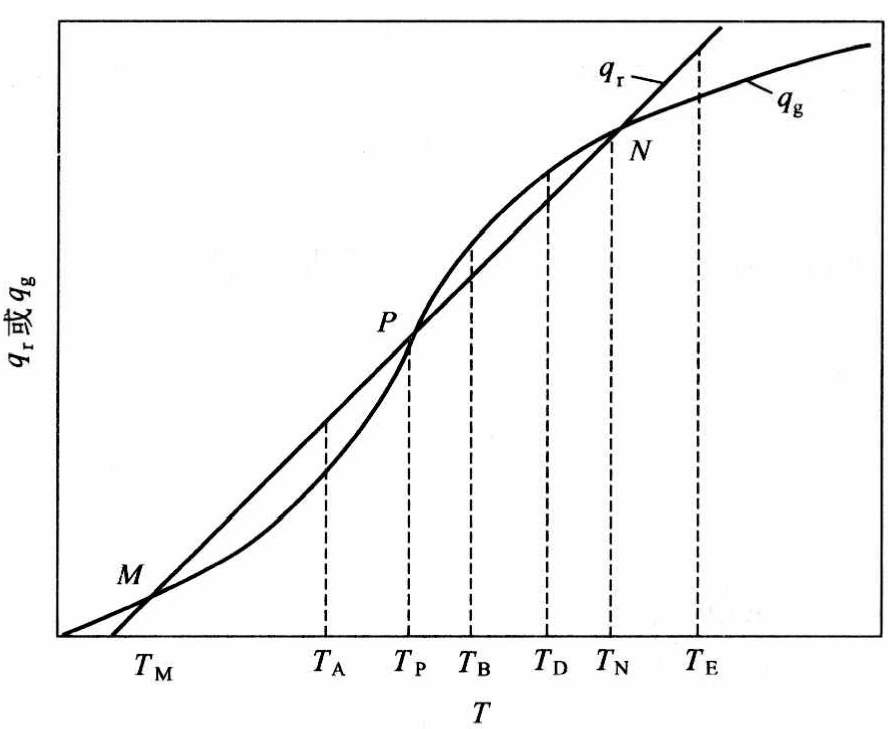
\includegraphics[width=\linewidth]{figs/fig3.13.png}
        \column{9.5cm}
            \begin{itemize}
            \item 移热速率线$q_\mathrm{r}$为一直线，斜率为$Q_{0} \rho \bar{C}_{p \mathrm{t}}+U A_{\mathrm{h}}$
            \item 放热速率曲线$q_\mathrm{g}$为一S形曲线
            \item 两线的交点的温度即为定态操作温度
            \end{itemize}        
    \end{columns}
\end{frame}


\begin{frame}
    \frametitle{连续釜式反应器的定态}

    \begin{columns}[c]
        \column{6cm}
            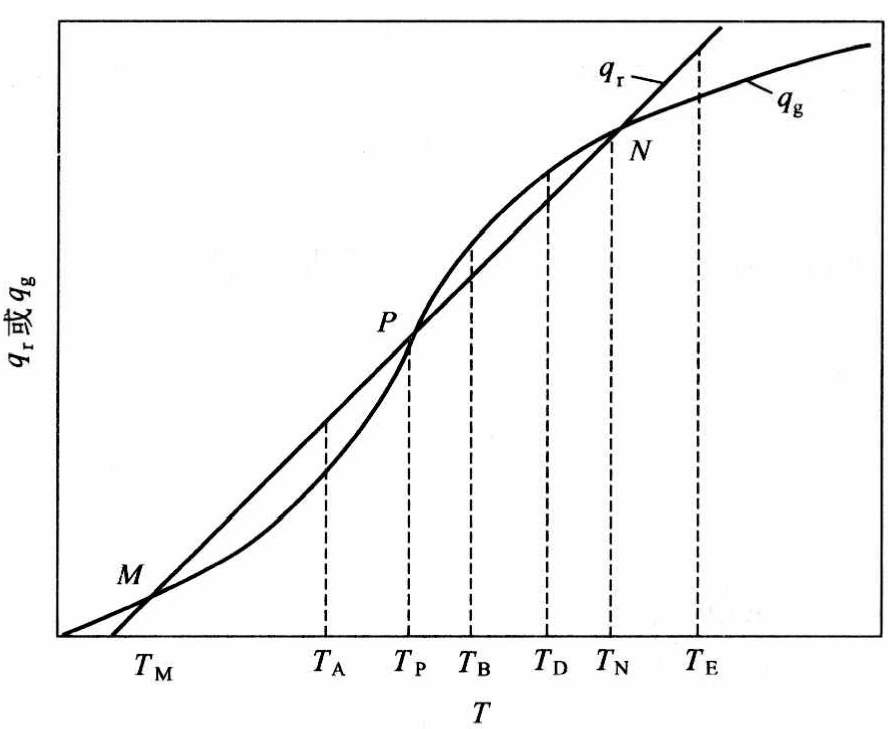
\includegraphics[width=\linewidth]{figs/fig3.13.png}
        \column{7.5cm}
            \begin{itemize}
            \item $T_\mathrm{M}$、$T_\mathrm{N}$、$T_\mathrm{P}$为定态操作温度
            \item 按$T_\mathrm{M}$操作，转化率最低，按$T_\mathrm{N}$操作，转化率最高            
            \item M、N为稳定定态点
            \item P为不稳定的定态点
            \item 只有放热反应才可能出现多定态现象，吸热反应的定态总是唯一的
            \end{itemize}        
    \end{columns}
    ~\\
    以N点为例，当受到外来干扰温度上升至$T_\mathrm{E}$，此时移热速率大于放热速率，扰动消除后，反应物系必然降温至$T_\mathrm{N}$。如由于外来干扰温度下降至$T_\mathrm{D}$，此时$q_\mathrm{r}$大于$q_\mathrm{g}$，扰动消除后，反应物系必然升温至$T_\mathrm{N}$。所以N是稳定定态点。

\end{frame}


\begin{frame}
    \frametitle{连续釜式反应器的着火点和熄火点}
    当进料流量一定且传热系数及反应物料的比热容可视为常数时，进料或换热介质温度改变只使移热曲线的位置发生变化，而不影响放热曲线。
    \vspace{6pt} 
    \begin{columns}[c]        
        \column{5.5cm}
        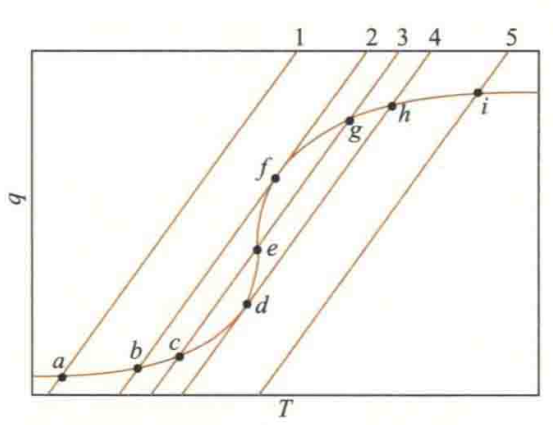
\includegraphics[width=\linewidth]{figs/fig3.14a.png}
        \centering 进料温度不同时的定态点
        \column{8cm}
        当进料温度从$T_1$慢慢地增加到$T_4$时，定态温度从点$a$变至$d$，该点为不稳定的定态点，只要进料温度稍微增加，定态点即从点$d$跳至点$h$出现不连续现象。这种情况称为着火，点d称为着火点。

        如逐渐降低进料温度，点$f$为不稳定的定态点，定态点将从点$f$跳至点$b$。这种情况称为熄火，点$d$称为熄火点。
    \end{columns}
\end{frame}


\begin{frame}
    \frametitle{连续釜式反应器的着火点和熄火点}
    \begin{columns}[c]
        \column{8cm}
            如图为进料温度$T_0$与定态温度$T$的关系示意图。
            
            当进料温度从$T_1$慢慢地增加至$T_5$时，定态温度的变化$a\rightarrow b\rightarrow c\rightarrow d\rightarrow h\rightarrow i$。
            
            曲线在$d$点处是不连续的，定态温度突然增高，这一点称为着火点；

            若将进料温度逐渐降低，比如从$T_5$降至$T_1$，定态温度则沿$i\rightarrow h\rightarrow g\rightarrow f\rightarrow b\rightarrow a$曲线下降。间断点$f$称为熄火点。
        \column{5.5cm}
            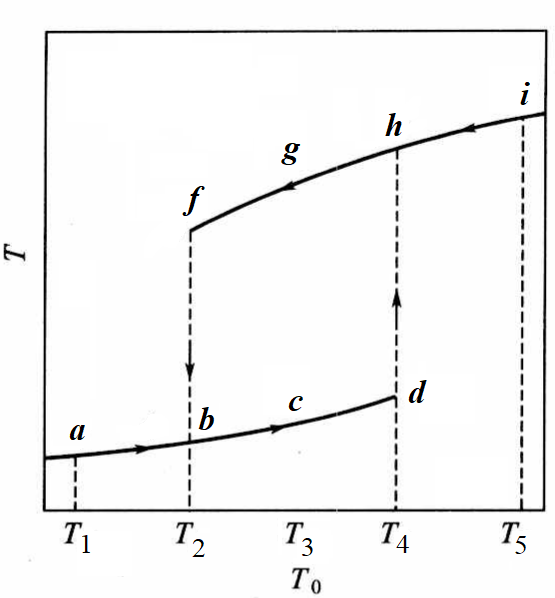
\includegraphics[width=\linewidth]{figs/fig3.14.png}
    \end{columns}    
    当进料温度在$T_2$与$T_4$的范围内时，则产生多定态现象。在此温度范围之外，定态温度是唯一的。
\end{frame}


\begin{frame}[t]{}
    \begin{example}
        温度为326K的顺丁烯二酸酐和正己醇的混合液，以\SI{0.01}{m^3/s}的流量连续地通入反应体积为\SI{2.65}{m^3}的绝热釜式反应器进行酯化反应
        \[
            \ce{C4H2O3 + C6H13OH -> HOOC-CH=CH-COO(C6H13)}
        \]
        该反应对顺丁烯二酸酐和正己醇均为一级，反应速率常数等于
        \[
            k = 1.37 \times 10^{12} \exp{(-12628/T)} \qquad \mathrm{m^3/(kmol \cdot s)}
        \]
        该反应的反应热为\SI{-33.5}{kJ/mol}，反应混合物的$\rho \bar{C}_{p \mathrm{t}}$可按\SI{1980}{kJ/(m^3.K)}计算。

        进料液中酐和醇的浓度分别为\SI{4.55}{kmol/m^3}和\SI{5.34}{kmol/m^3}，试计算反应器出口转化率及温度。
    \end{example}

\end{frame}





\begin{frame}[t]{}
    \vspace{-9pt}
    \begin{block}{习题3.22}
        在反应体积为\SI{0.75}{m^3}的全混流反应器中进行醋酐水解反应，进料体积流量为0.05 \si{m^3/min}，醋酐浓度为\SI{0.22}{kmol/m^3}，温度为25℃，出料温度为36℃。该反应为一级不可逆放热反应，反应热效应等于\SI{-209}{kJ/mol}，反应速率常数
        \[
            k=1.8 \times 10^7 \exp{-5526/T} \qquad 1/\mathrm{min}
        \]
        反应物料的密度为常数，等于\SI{1050}{kg/m^3}，热容可按\SI{2.94}{kJ/(kg.K)}计算。该反应器没有安装换热器，仅通过反应器壁向大气散热。试计算：(1)反应器出口物料中醋酐的浓度；(2)单位时间内反应器向大气散出的热量。
        \tcblower
        \only<1>{
            ~

            ~

            ~
        }
    \only<2>{
        \begin{align*}
            V_{r}&=\frac{Q_{0} X_{A f}}{k(1-X_{A f})}=\frac{0.05 X_{A f}}{0.308(1-X_{A f})}=0.75 \qquad \qquad X_{A f} = 0.8221\\        
            C_{A}&=C_{A 0}(1-X_{A})=0.22(1-0.8221)=0.03914 \mathrm{kmol} / \mathrm{m}^{3}        
        \end{align*}
    }
    \only<3>{
    \[
        \begin{aligned}
             Q^{\prime}&=Q_{0} \rho \bar{C}_{p t}(T-T_{0})+(\Delta H_{r})(-R_{A}) V_{r} \\
            &=0.05 \times 1050 \times 2.94(309-298)+(-209000) 0.308 \times 0.22(1-0.8221) 0.75\\
            &=-191 \mathrm{~kJ} / \mathrm{min}
        \end{aligned}
    \]
    }
    \end{block}
\end{frame}






















\end{document}